\documentclass{beamer}

\usepackage{beamerthemesplit}

\usetheme{Boadilla} 

\usepackage[utf8]{inputenc}
\usepackage[T1]{fontenc}
\usepackage[utf8]{vietnam}
\usepackage[english]{babel}
\usepackage{calc}
\usepackage{ifthen}
\usepackage{tikz}
\usepackage{eurosym}

\usepackage{alltt}

\usepackage{verbatim}

\usepackage[french,algoruled,vlined,noend]{algorithm2e}
\SetKwIF{Si}{SinonSi}{Sinon}{si}{}{sinon si}{sinon}{}
\SetKwFor{Pour}{pour}{}{}
\SetKwFor{RepeterNFois}{répéter}{fois}{}
\SetKwFor{TantQue}{tant que}{}{}%
\SetKwFor{PourChaque}{pour chaque}{}{}%

\usepackage{CJKutf8}

\usepackage[overlap, CJK]{ruby}
\usepackage{CJKulem}

\renewcommand{\rubysep}{-0.2ex}

\newenvironment{SChinese}{%
  \CJKfamily{gbsn}%
  \CJKtilde
  \CJKnospace}{}
\newenvironment{TChinese}{%
  \CJKfamily{bsmi}%
  \CJKtilde
  \CJKnospace}{}
\newenvironment{Japanese}{%
  \CJKfamily{min}%
  \CJKtilde
  \CJKnospace}{}
\newenvironment{Korean}{%
  \CJKfamily{mj}}{}
  
\newcommand{\cntext}[1]{\begin{CJK}{UTF8}{}\begin{Japanese}#1\end{Japanese}\end{CJK}}

\pgfdeclareimage[height=0.8cm]{logo}{img/getalp}
\pgfdeclareimage[height=1.5cm]{logobig}{img/getalp} 

\logo{\pgfuseimage{logo}}

\title{Dbnary: wiktionary et le web lexical}
\subtitle{Wiktionnaire, RDF, Linked Data: une colonne vertébrale pour le lexique ?}
\author{Gilles Sérasset}
\institute[GETALP-LIG]{GETALP-LIG, Université Joseph Fourier, Grenoble, France}
\titlegraphic{\pgfuseimage{logobig}}
\date{\today}

% Delete this, if you do not want the table of contents to pop up at
% the beginning of each subsection:
\AtBeginSection[]
{
  \begin{frame}<beamer>
    \frametitle{}
    \tableofcontents[currentsection]
  \end{frame}
}

\begin{document}

\frame{\titlepage}


\section{Introduction}

\frame{\frametitle{Propos liminaires}
\centering{Cette présentation à été préparée avec une méthode \alert{ancestrale}...\\
~\\
\pause
C'est la méthode \alert{ALARACHE !}!\\
~\\
Cela signifie que je compte sur vous! Rendez la vivante et complète en m'interrompant!\\
~
Ou nous nous ferons tous \only<2>{\alert{Magn}(ennuyer)}\only<3>{ch... comme la mort (bored to death)}\\}
}

\frame{\frametitle{Qui suis je ?}
\centering{Je travaille sur la structuration/gestion/... des bases lexicales multilingues (MLDB) depuis 1990.\\
~\\
Thèse: définition d'une approche pivot pour les MLDB et d'un système générique de gestion des MLDB (1994)\\
~\\
Responsable projet Papillon depuis 2000.\\
}
}

\frame{\frametitle{Mes contributions principales ?}
\begin{itemize}
\item Approche par acceptions interlingues (Axies)
	\begin{itemize} 
	\item évite les biais de l'utilisation d'une langue naturelle comme pivot
	\item Reprise dans le standard Lexicon Markup Framework 
	\end{itemize}
\item Outils génériques pour les MLDB\\
	\begin{itemize} 
	\item plateforme JIBIKI
	\item utilisée pour le projet Papillon
	\item réutilisée (ainsi que l'approche par acception) pour le projet LexALP 
	\item ... GDEF, DILAF (Mathieu Mangeot)
	\end{itemize}
\item Réflexion sur les lexiques, leur acquisition
	\begin{itemize} 
	\item Modèle de graphes: Lexical systems,
	\item corpus vu comme un graphe
	\item extraction d'informations lexicales vu comme des opérations sur des graphes 
	\item ... Thèse de Vincent Archer
	\end{itemize}
\end{itemize}
}

\section{Apparté: le projet Papillon}

\frame{
  \frametitle{Overview of the Papillon Project}
  \begin{itemize}
    \item Initialy launch by a French Japanese consortium (2000)
    \item Quickly extended itself to a larger consortium
   \begin{itemize}
    \item with partners in Australia, Canada, China, France, Germany, Japan, Malaysia, Thailand, Vietnam\ldots
    \item \ldots and accepting any new partner motivated enough to join the adventure... 
  \end{itemize}
  \item Aims at the development of a rich, ``open source'', multilingual lexical database
  \end{itemize}
}

\frame{
  \frametitle{Architecture of the Data}
  \framesubtitle{Macrostructure: An acception based multilingual lexical database}
  
  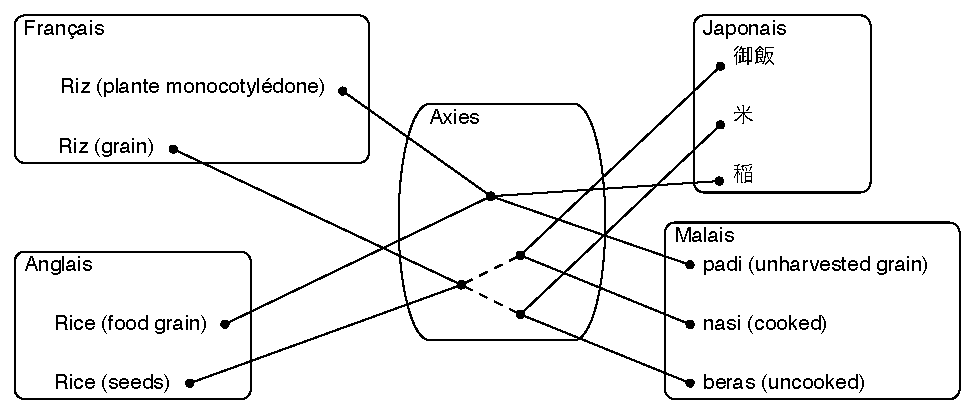
\includegraphics[width=\linewidth]{figs/axies.pdf}
}

\frame{
  \frametitle{Architecture of the Data}
  \framesubtitle{A microstructure inspired by Mel'\v{c}uk's ECD and Polguère's DICO}
  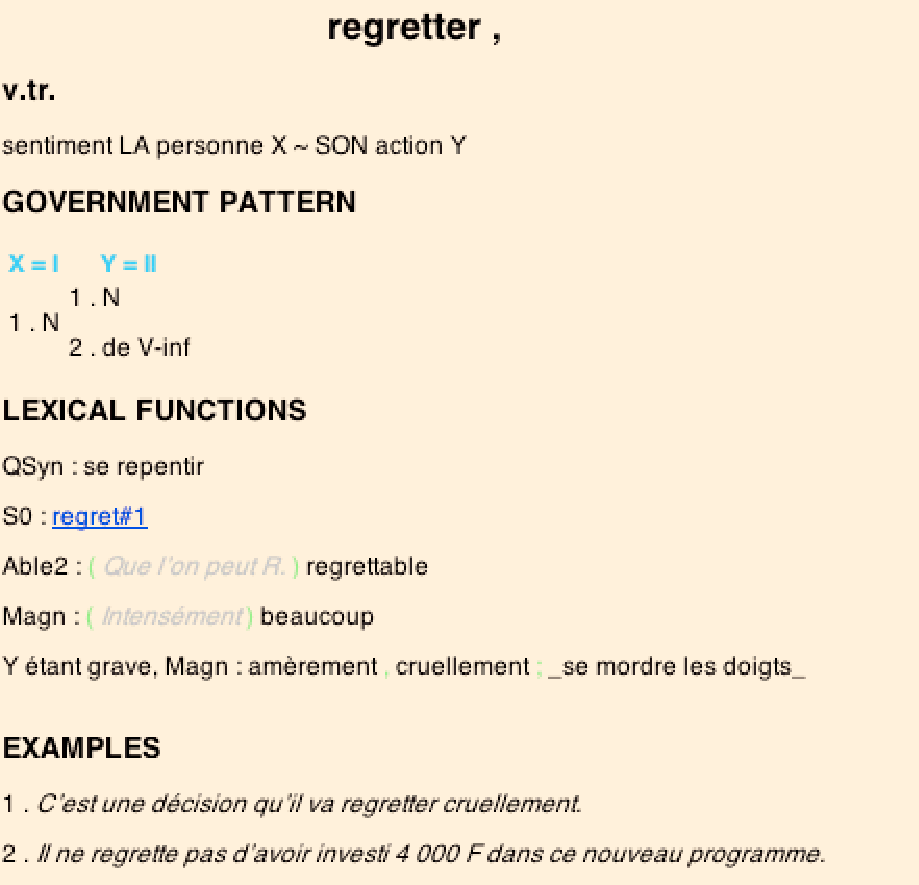
\includegraphics[height=7cm]{figs/regretter-expanded.pdf}
}

\section{État actuel de mes réflexions}

\frame{\frametitle{Mes réflexions actuelles}
\begin{itemize}
\item Interopérabilité "syntaxique"
	\begin{itemize} 
	\item Biais d'XML dans jibiki
	\item ... Passage en RDF...
	\item ... Lexical Linked Data.
	\end{itemize}
\item Interopérabilité "sémantique"\\
	\begin{itemize} 
	\item Relier/aligner les sens de différentes resources
	\item techniques proches du WSD
	\item Besoin de sens décrits, \alert{avec des définitions} 
	\item ... difficulté d'en construire.
	\end{itemize}
\item Multilinguisme
	\begin{itemize} 
	\item modèle par acceptions toujours d'actualité
	\item besoin de bases lexicales multilingues encore d'actualité (même si on est passé d'une disette à une sur-abondance d'information lexicale)
	\item importance des informations adjectivales, verbales, adverbiales 
	\item focalisation du domaine sur le nominal (wikipedia)
	\end{itemize}
\end{itemize}
}

\section{Dbnary}

\frame{\frametitle{Dbnary: une première action}
\begin{itemize}
\item Un grand dictionnaire, gratuit, avec des définitions ?
	\begin{itemize} 
	\item Wiktionary
	\end{itemize}
\item Intéropérabilité "à grain fin"\\
	\begin{itemize} 
	\item RDF
	\end{itemize}
\item Un modèle standard
	\begin{itemize} 
	\item LEMON (inspiré de LMF)
	\end{itemize}
\item Multilingue
	\begin{itemize} 
	\item extraction de plusieurs "language edition" de Wiktionary
	\end{itemize}
\item Disponible, utilisable et utilisé
	\begin{itemize} 
	\item Linked Data
	\end{itemize}
	
\end{itemize}
}

\frame{  
\frametitle{Dbnary: Wiktionary comme graphe lexical}

     \includegraphics<1>[width=\linewidth]{figs/cat1.png}
     \includegraphics<2>[width=\linewidth]{figs/cat2.png}
     \includegraphics<3>[width=\linewidth]{figs/cat3.png}
     \includegraphics<4>[width=\linewidth]{figs/cat4.png}
     \includegraphics<5>[width=\linewidth]{figs/cat5.png}
     \includegraphics<6>[width=\linewidth]{figs/cat6.png}
     \includegraphics<7>[width=\linewidth]{figs/cat_struct}
     \includegraphics<8>[width=\linewidth]{figs/cat_syn}
     \includegraphics<9>[width=\linewidth]{figs/cat_translations}

}

\frame{  
\frametitle{LEMON}

     \includegraphics<1>[width=\linewidth]{figs/lemon-core.png}
     \includegraphics<2>[width=\linewidth]{figs/lemon-descr.png}
     \includegraphics<3>[width=\linewidth]{figs/dbnary-lemon-xtension.pdf}

}

\frame{
\frametitle{Principe d'extraction}
\begin{itemize}
\item 8 éditions extraites: en, fr, de, ru, it, pt, fi, el
\item Extraction à partir des dumps de wikimedia
\item Chaque édition met à jour son dump tous les 10-15j
\item l'extraction est faite en direct, les fichiers sont accessibles en ligne immédiatement
\item le serveur "Linked Data" contient des données plus anciennes
\end{itemize}
}

\frame{  
\frametitle{Taille des données (aujourd'hui)}

\begin{table}[htb]
\begin{tabular}{lrrrr}
 & \textbf{Entries} & \textbf{Vocables} & \textbf{Senses} & \textbf{Translations}\\
 \hline
\textbf{eng} & 527067 & 504594 & 421232 & 1126463 \\
\textbf{fra} & 273822 & 283847 & 358921 & 464956 \\
\textbf{deu} & 135103 & 201736 & 95593 & 471892 \\
\textbf{rus} & 127271 & 139235 & 99243 & 325345 \\
\textbf{ell} & 74056 & 74800 & 34932 & 55652 \\
\textbf{fin} & 48164 & 48050 & 56559 & 118728 \\
\textbf{por} & 43042 & 44061 & 77631 & 225065 \\
\textbf{ita} & 25279 & 31935 & 35061 & 57796 \\
\end{tabular}
\caption{Number of resources by type and language, sorted by number of lexical entries.}\label{globalsize}
\end{table}
}

\frame{  
\frametitle{Taille des données (aujourd'hui)}
\begin{table}[htb]
\begin{tabular}{lrrrrrr}
 & \textbf{syn}  & \textbf{ant} & \textbf{hyper} & \textbf{hypo} & \textbf{mero} & \textbf{holo} \\
 \hline
\textbf{eng} & 31461& 6877& 959& 1103& 114& 0 \\ 
\textbf{fra} & 30088& 6735& 8215& 3557& 943& 1847 \\ 
\textbf{deu} & 27516& 14315& 30202& 9509& 0& 0 \\ 
\textbf{rus} & 22631& 9204& 21028& 4756& 0& 0 \\ 
\textbf{ell} & 3975& 1116& 0& 0& 0& 0 \\ 
\textbf{fin} & 2255& 0& 0& 0& 0& 0 \\ 
\textbf{por} & 3527& 575& 6& 3& 0& 0 \\ 
\textbf{ita} & 7091& 2337& 0& 0& 0& 0 \\ 
\end{tabular}
\caption{Number of lexicon-semantic relations. Languages are sorted according to their number of lexical entries.}\label{nymsize}
\end{table}
}

\frame{  
\frametitle{Taille des données (aujourd'hui)}
\begin{table}[htb]
\begin{tabular}{lrrrrrrrrrrrrr}
\textbf{Source/Target}  & \textbf{deu} & \textbf{ell} & \textbf{eng} & \textbf{fin} & \textbf{fra} & \textbf{ita} & \textbf{por} & \textbf{rus}& \textbf{others} & \textbf{Total} & \textbf{\# of target languages}\\
\textbf{eng} & 62501 & 23794 & 1 & 74938 & 57959 & 37467 & 30256 & 74837 & 764710 & 1126463 & 1143\\
\textbf{fra} & 34608 & 7063 & 74687 & 7589 & 12 & 18806 & 17784 & 7783 & 296624 & 464956 & 952\\
\textbf{deu} & 0 & 2675 & 81015 & 4947 & 67143 & 41485 & 8872 & 17354 & 248401 & 471892 & 355\\
\textbf{rus} & 23056 & 3295 & 48559 & 3966 & 14776 & 12643 & 5567 & 0 & 206709 & 318571 & 490\\
\textbf{ell} & 2242 & 2 & 10090 & 1056 & 8436 & 1470 & 1149 & 1315 & 29892 & 55652 & 246\\
\textbf{fin} & 8046 & 918 & 30103 & 0 & 6700 & 3856 & 2196 & 7997 & 58912 & 118728 & 329\\
\textbf{por} & 7000 & 2816 & 11284 & 4607 & 8720 & 7096 & 4 & 4396 & 179142 & 225065 & 695\\
\textbf{ita} & 4619 & 506 & 17539 & 925 & 4461 & 75 & 1219 & 938 & 27514 & 57796 & 315\\
\end{tabular}
\caption{Number of translations from/to the 8 currently extracted languages. Source languages are sorted according to their number of lexical entries. Target languages are sorted by their ISO 639-3 language code. The number of different target languages is also given.}\label{tradsize}
\end{table}
}

\frame{  
\frametitle{Taille des données (aujourd'hui)}
\begin{table}[htb]
\begin{tabular}{lrrrrrr}
\textbf{Source/Target}  & \textbf{por} & \textbf{rus}& \textbf{others} & \textbf{Total} & \textbf{\# of lang}\\
\textbf{eng} & 30256 & 74837 & 764710 & 1126463 & 1143\\
\textbf{fra} & 17784 & 7783 & 296624 & 464956 & 952\\
\textbf{deu} & 8872 & 17354 & 248401 & 471892 & 355\\
\textbf{rus} &  5567 & 0 & 206709 & 318571 & 490\\
\textbf{ell} &  1149 & 1315 & 29892 & 55652 & 246\\
\textbf{fin} &  2196 & 7997 & 58912 & 118728 & 329\\
\textbf{por} &  4 & 4396 & 179142 & 225065 & 695\\
\textbf{ita} &  1219 & 938 & 27514 & 57796 & 315\\
\end{tabular}
\caption{Number of translations from/to the 8 currently extracted languages. Source languages are sorted according to their number of lexical entries. Target languages are sorted by their ISO 639-3 language code. The number of different target languages is also given.}\label{tradsize}
\end{table}
}

\frame{  
\frametitle{Qualité des données}

\begin{itemize}
\item Évaluer la qualité des données est difficile
\item Qualité de l'extraction $\ne$ qualité des données
\item Pas d'application particulière actuellement
\item Pas encore d'alignement avec d'autres ressources (wordnet, jeuxdemots, ...)
\item Mais quelques indices...
\end{itemize}
}

\frame{  
\frametitle{Qualité des données (hier)}
\begin{table}[htb]
\begin{tabular}{lrr}
\textbf{language} & \textbf{\# of transl.}\\
 \hline
\textbf{eng} & 5110 (99.1 \%) \\
\textbf{fra} & 5799 (107.0 \%) \\
\textbf{deu} & 10287 (99.2 \%)\\
\textbf{rus} & 8436 (24811.7 \%) \\
\textbf{ell} & 2598 (64.3 \%) \\
\textbf{fin} & 7245 (28980 \%) \\
\textbf{por} & 17720 (93.2 \%) \\
\textbf{ita} & 7855 (3167.3 \%) 
\end{tabular}
\caption{Extracted translations vs interwiki links, on a random sample of 1000 entries.}\label{iwlinks}
\end{table}
}

\section{RDF, Linked data, késako ?}

\frame{  
\frametitle{RDF: Resource Description Framework}

\centering{Un graphe = un ensemble de \alert{Statements}\\
~\\
un statement = un triplet: (S, P, O)\\
~\\
\only<2>{S: forcément une URI; P: une URI; O: une URI ou un littéral}~\\
\only<3>{\alert{Attention}: une URI n'est pas forcément une document URL}~\\
~\\
     \includegraphics<1>[width=\linewidth]{figs/rdf-sample-generic.pdf}
     \includegraphics<2>[width=\linewidth]{figs/rdf-sample-uri.pdf}
     \only<3>{\texttt{http://getalp.imag.fr/Journée\_LIG-LIDILEM} : EROR 404: Not found !}
}
}

\frame{  
\frametitle{RDF: Resource Description Framework}

\centering{Comment représenter un document RDF ?\\
~\\
RDF est un modèle, pas une syntaxe...\\
~\\
On le confond souvent avec RDF+XML une syntaxe absconse...\\
~\\
Mais il y a des tas de manière de transférer des données RDF: Turtle, N3, HTML+RDFa...\\
Les outils les comprennent souvent toutes...\\
}
}

\frame{  
\frametitle{RDF: Resource Description Framework}

{Exemple en turtle...\\
~\\
}
\texttt{@prefix getalp: <http://getalp.imag.fr/>\\
@prefix sem: <http://seminaires.fr/38/>\\
@prefix dcterm: <http://purl.com/dcterm>\\
~\\
getalp:Journée\_LIG-LIDILEM\\
~~~~dcterm:date "2 juillet 2013"@fr\\
~~~~dcterm:lieu sem:chateau\_commanderie .}
}

\frame{  
\frametitle{RDF: Resource Description Framework}

\centering{Quoi d'autre ?\\
~\\
On peut aussi décrire les meta-donnée en RDF (OWL) \\
~\\
par exemple: \\
~~l'objet d'une relation "lieu" est forcément un lieu géographique.\\
~~un "dcterm:event" a forcément une date, un lieu et au moins un participant...\\
~\\
~~Un raisonnement est possible:\\
~~~~\texttt{getalp:Journée\_LIG-LIDILEM a dcterm:event}\\
~~~~implique qu'il existe un participant...\\
}
}

\frame{  
\frametitle{RDF: Resource Description Framework}

\centering{Quoi d'autre ?\\
~\\
De nombreux outils existent \\
~\\
par exemple: \\
Bases de données spécialisées (virtuoso, JENA, Sesame, etc...)\\
Langage de requêtes: SPARQL\\
Raisonneurs\\
}
}

\frame{  
\frametitle{Et le "Linked Data" ? Koikesse ?}

\centering{En gros (très gros), les URIs deviennent des URLs\\
~\\
On peut donc "résoudre" (déréférencer) les noeuds de l'arc \\
~\\
Tout se passe comme si chaque noeud était à la foi \\
un objet du modèle... (comme en RDF)\\
une page web décrivant l'objet pour un utilisateur...\\
un document RDF décrivant l'objet pour un outil du web sémantique\\
~\\
C'est le serveur web qui "négocie" et redirige vers l'info adéquate.\\
}
}

\frame{  
\frametitle{Et le "Linked Data" ? safékoi ?}

\centering{Si les données sont disponibles sur les serveurs, il est inutile de les avoir "en local"...\\
~\\
Elles sont dispersées\\
~\\
On peut donc utiliser des données qu'on n'a pas "chez soi".\\
}
}



\section{Conclusion}

\frame{  
\frametitle{Conclusion}

\begin{itemize}
\item Il reste des données à construire (langues peu dotées, collocations, etc)
\item Mais pour les grandes langues, c'est l'abondance
\item Besoin fort actuel: l'interopérabilité
\item Une réponse: le Lexical Linked Data
\item Une ressource à laquelle "attacher" les autres données: dbnary
\item Suite: désambiguïser pour "monter" les relations au niveau des sens
\item Suite: faire émerger un pivot lexical non linguo-centré
\item Suite: aligner aver d'autres resources RDF (Wordnet, JeuxDeMots (trivial à RDFiser), ...)
\end{itemize}
}


\end{document}




%%%%%%%%%%%%%%%%%%%%%%%%%%%%%%%%%%%%%%%%%%%%%%%%%%%%%%%%%%%%%%%%%%

\part{Multilingual Lexical Resources, a First Approach}
\frame{\partpage}

\section{Dictionaries and Other Lexical Data}

% What you see on a paper dictionary, how is each entry structured ?
% How can we represent such information in computers


\subsection{Monolingual Lexical Data}

\frame{
Monolingual  Lexical Data
}


\frame{\frametitle{Dictionary}
\begin{beamerboxesrounded}{A First Definition}
   A dictionary is a \alert<2>{book} of \alert<4>{alphabetically listed} \alert<2>{words} in a specific language, \alert<3>{with definitions, etymologies, 
pronunciations, and other information}; or a \alert<2>{book} of \alert<4>{alphabetically listed} \alert<2>{words} in one language with their 
equivalents in another, also known as a lexicon.\footnote{Webster's New World College Dictionary, Fourth Edition, 2002}
\end{beamerboxesrounded} 

\begin{enumerate}
\item<2-> a collection of \alert{words},
\item<3-> each word comes with a \alert{set of information} that describe it,
\item<4-> there is an implicite \alert{access method} to each word.
\end{enumerate}
}

\frame{
\frametitle{Examples of monolingual dictionary}
\pgfdeclareimage[width=\linewidth]{dict}{img/composedict}
\pgfdeclareimage[width=\linewidth]{dict2}{img/composedict2}
\pgfuseimage{dict}\\
\pause
\pgfuseimage{dict2}
}

\frame{\frametitle{Thesaurus}
\begin{beamerboxesrounded}{A First Definition}
   A Thesaurus is a listing of \alert<2>words with similar, related, or opposite meanings (this new meaning of thesaurus dates back to Roget's Thesaurus)
\end{beamerboxesrounded} 

\begin{enumerate}
\item<2-> a collection of \alert{words},
\item<3-> there are no definition or description of each word (this is left to the dictionary),
\item<4-> a thesaurus may be seen as a network of word \alert{senses}.
\end{enumerate}
}

\frame{
\frametitle{An example of monolingual thesaurus}
\pgfdeclareimage[width=\linewidth]{thes}{img/composethes}
\only<1>{\pgfuseimage{thes}}
}

\frame{\frametitle{A first set of problems}

  \begin{beamerboxesrounded}{What is a word ?}
    \begin{itemize}
    \item \textit{Composed} and \textit{Compose}: one or two words ?
    \item \textit{Compose} and \textit{Composition}: one or two words ?
    \end{itemize} 
  \end{beamerboxesrounded}

\pause
  \begin{beamerboxesrounded}{Different dictionaries do not agree on the granularity of lexical entries}
    \begin{itemize}
    \item \textit{Stock$_{v}$} and \textit{Stock$_{n}$}: one or two entries ?
    \item \textit{Judgement$_{judging}$} and \textit{Judgement$_{estimate}$}: one or two word senses ?
    \end{itemize}
  \end{beamerboxesrounded}

\pause
  \begin{beamerboxesrounded}{How does different lexical data interoperate ?}
    \begin{itemize}
    \item Can I merge information from the dictionary and from the thesaurus ?
    \item Can I merge information from two different dictionaries ?
    \end{itemize}
  \end{beamerboxesrounded}

\pause
  \begin{beamerboxesrounded}{Can I extract data from a dictionary ?}
    \begin{itemize}
    \item How is the dictionary structured ?
    \item How is this structure represented ?
    \item Are definitions consistant ?
    \end{itemize}
  \end{beamerboxesrounded}

}


\subsection{Bilingual Lexical Data}

\frame{
  Bilingual Lexical Data
}

% same as monolingual dictionaries
\frame{\frametitle{Bilingual Dictionary: an example}
\pgfdeclareimage[width=.8\linewidth]{dictenfr}{img/composeenfr}
\pgfuseimage{dictenfr}

~

\pgfdeclareimage[width=\linewidth]{dictenfr2}{img/composeenfr2}
\pgfuseimage{dictenfr2}
}

\frame{\frametitle{A second set of problems}

  \begin{beamerboxesrounded}{How do I translate in my context?}
    \begin{itemize}
    \item What is my word sense?
    \item What is the resulting word sense ?
    \end{itemize} 
  \end{beamerboxesrounded}

\pause
  \begin{beamerboxesrounded}{Can I use this info to translate the other way round?}
    \begin{itemize}
    \item How much of the word sense is covered by the translation ?
    \item How marginal is the target word sense, compared to word senses of the target word ?
    \end{itemize}
  \end{beamerboxesrounded}
}


\subsection{Multilingual Lexical Data}

\frame{
Multilingual Lexical Data
}
% No real printed multilingual dictionaries, merely a collection of bilingual dictionaries
% Exception for terminological data: why ?

\frame{\frametitle{An example of multilingual terminological database}
\pgfdeclareimage[width=\linewidth]{unterm}{img/unterm}
\pgfuseimage{unterm}
}

\frame{\frametitle{An example of a multi-bilingual dictionary}
\pgfdeclareimage[width=\linewidth]{fem}{img/fem}
\pgfuseimage{fem}
}

\frame{\frametitle{Did you ever use a \alert{really} multilingual printed dictionary ?}

I mean: a dictionary for which you can use ANY language as a source and ANY language as a target...

\pause

~

No ?

~

  \pause 
That's normal... such dictionary do not exist...

... because nobody knows how to layout/present such information on paper... 

... except in very specific situations (i.e. terminology)

\pause
~

But you may find such a database online.
}

\frame{\frametitle{
    \begin{center}
      Before we go further, let's see what are the technical difficulties that has to be handled...
    \end{center}
}}

\section{Computational Problems posed by ALL Lexical Data}

\subsection{Denoting languages of the world}

\newcounter{temp}


% calculate the anchor of the external label
\newcommand{\angledir}[1]{
  \setcounter{temp}{#1}

  \ifthenelse{\thetemp < 0}{\addtocounter{temp}{360}}{}
  \ifthenelse{\thetemp > 360}{\addtocounter{temp}{-360}}{}

  \ifthenelse{\thetemp < 11}{\def\piedir{right}}{
  \ifthenelse{\thetemp < 80}{\def\piedir{above right}}{
  \ifthenelse{\thetemp < 101}{\def\piedir{above}}{
  \ifthenelse{\thetemp < 170}{\def\piedir{above left}}{
  \ifthenelse{\thetemp < 191}{\def\piedir{left}}{
  \ifthenelse{\thetemp < 260}{\def\piedir{below left}}{
  \ifthenelse{\thetemp < 281}{\def\piedir{below}}{
  \ifthenelse{\thetemp < 350}{\def\piedir{below right}}{
    right}}}}}}}}%
}

% calculate the position of the internal label
\newcommand{\calcpiedist}[1]{%
  \ifthenelse{#1 > 120}{\def\piedist{0.50}}{
  \ifthenelse{#1 < 10}{\def\piedist{0.80}}{
    \setcounter{temp}{(80 * (120-#1) + 50 * (#1-10))/110}
    \def\piedist{0.\thetemp}}}
}

% draw a slice of a pie chart
% The diffI and diffII counters are just a quick hack for making the
% code compatible with PGF 1.18
% The code should be rewritten to utilize the new math engine.
\newcounter{diffI}
\newcounter{diffII}
\newcommand{\slice}[4]{%
  \setcounter{temp}{(#1+#2)/2}
  \setcounter{diffI}{#1-\thetemp}
  \setcounter{diffII}{#2-\thetemp}
  \begin{scope}[rotate=\thetemp]
  %\pgfmathparse{#1-\thetemp}
    \draw[fill=black!10,join=round,thick]
                                (0,0)
                             -- (\thediffI:1cm)
                             arc (\thediffI:\thediffII:1cm)
                             -- cycle;
    \angledir{\thetemp}
    \node [\piedir] at (1,0) {#4};
    \setcounter{temp}{#2-#1}
    \calcpiedist{\thetemp}
    \node at (\piedist,0) {#3};

  \end{scope}
}


\frame
{
  \frametitle{Languages of the world}
  
  The biggest database on the matter is the ``Ethnologue\footnote{http://www.ethnologue.com/}'' database. It currently contains 6912 \emph{living} languages in the world that are geographically distributed as:
    
  \begin{tikzpicture}[scale=3]

\newcounter{a}
\newcounter{b}
\foreach \p/\t in {16/America, 30/Africa, 3/Europe,
                   32/Asia, 19/Pacific}
  {
    \setcounter{a}{\value{b}}
    \addtocounter{b}{\p}
    \slice{360*\thea/100}
          {360*\theb/100}
          {\p\%}{\t}
  }
\end{tikzpicture}
}

\frame{
	\pgfdeclareimage[height=7cm]{lgmonde}{img/WRLD_ETH_CROPPED} 
	\pgfuseimage{lgmonde}
	
	\footnotesize{image taken from http://www.ethnologue.com/}
}

\frame
{
  \frametitle{Languages of the world (cont.)}
  
  This distribution is the result of difficult work and the precision of the numbers is not easy to evaluate. The problems are:
  \begin{itemize}
  \item Heterogeneity of the sources
  \item The difficult distinction between langages and dialecte.\footnote{languages are generally the object of statistics, but the definition of a language is based on subjective and variable criteria.}
  \end{itemize}
  Depending on the sources, estimations vary between about 3000 and 7000 living languages.
  
  ~
  
  \begin{beamerboxesrounded}{Max Weinreich}
  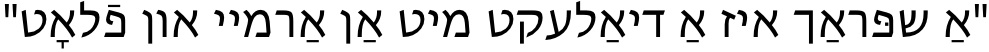
\includegraphics[height=1em]{img/weinreich}\\
  (a shprakh iz a dialekt mit an armey un flot)\\
  \emph{a language is a dialect with an army and a navy.}
  \end{beamerboxesrounded}
}

\frame
{
  \frametitle{Written languages, spoken languages}
  
  It is even more difficult to know the number of written languages. Depending on sources, 67\% to 90\% of the languages are spoken languages. This gives around 1500 written languages on the 6912.
  
  The bible society\footnote{www.biblesociety.org}  indicates that that the bible has been translated into 2426 different languages (at least one of the book has been translated).
  
  Certain languages, considered as oral languages can be written using a \emph{transcription} using an existing alphabet.

}


\frame{
\frametitle{Most spoken languages}
\footnotesize{
\begin{tabular}{lp{.25\textwidth}p{.4\textwidth}l}
\hline
Chinese & sino-tibétain & Chine & 885\\
\hline
English&indo-européen (groupe germanique)&Amérique du Nord, Grande-Bretagne, Australie, Afrique du Sud&450\\
\hline
Hindi-urdu&indo-européen (groupe indo-iranien)&Inde, Pakistan&333\\
\hline
Spanish&indo-européen (groupe roman)&Amérique du Sud, Espagne&266\\
\hline
Portuguese&indo-européen (groupe roman)&Brésil, Portugal, Angola, Mozambique&175\\
\hline
Bengali&indo-européen (groupe indo-iranien)&Bengladesh, Inde&162\\
\hline
Russian&indo-européen (groupe slave)&ex-URSS&153\\
\hline
Arabic&afro-asiatique&nord de l'Afrique, Moyen-Orient&150\\
\hline
Japanese&altaïque&Japon&126\\
\hline
French&indo-européen (groupe roman)&France, Canada, Belgique, Suisse, Afrique noire&122\\
\hline
\end{tabular}
}
}

\frame{
\frametitle{Most spoken languages}
\footnotesize{
\begin{tabular}{lp{.25\textwidth}p{.4\textwidth}l}
\hline
German&indo-européen (groupe germanique)&Allemagne, Autriche, Suisse&118\\
\hline
Wu&sino-tibétain&Chine (Chang-haï)&77\\
\hline
Javanese&austronésien&Indonésie (Java)&75\\
\hline
Korean&altaïque&Corée&72\\
\hline
Italian&indo-européen (groupe roman)&Italie&63\\
\hline
Marathi&indo-européen (groupe indo-iranien)&Inde du Sud&65\\
\hline
Telugu&dravidien&Inde du Sud&55\\
\hline
Tamoul&dravidien&Inde du Sud, Sri Lanka&48\\
\hline
Cantonese&sino-tibétain&Chine (Canton)&47\\
\hline
Ukrainian&indo-européen (groupe slave)&Ukraine&46\\
\hline
\end{tabular}
}
}


\subsection{Writing Systems}
\frame
{
  \frametitle{Writing Systems}
  
  Writing appeared under different forms in different human civilizations: egypt, Mesopotamia, China, India and, later, mid-america.
  
  The most ancient writing seams to be Mesopotamia, around 3500-3400 B.C.
  
  \begin{beamerboxesrounded}{}
	We use the term \emph{writing system}.
  \end{beamerboxesrounded}
  
  Two main classes:
  \begin{itemize}
  \item Phonologic Writings where \emph{phonemes} are written (alphabets + syllabaries)
  \item Semantic writings where \emph{morphemes} are written (Chinese writings, hieroglyphs or cuneiforms)
  \end{itemize}
}

\frame{
	\pgfdeclareimage[height=7cm]{writingsys}{img/WritingSystemsOfTheWorld} 
	\pgfuseimage{writingsys}
	
	\footnotesize{image taken from wikipedia}
}

\frame{
	\frametitle{Some examples}
	
	\begin{CJK}{UTF8}{}
	Japanese writing system:\\
	\begin{beamerboxesrounded}{}
	\begin{Japanese}
	UNICODE漢字コード分かりません。
	\end{Japanese}
  \end{beamerboxesrounded}
	\end{CJK}
	
	This system uses:
	\begin{itemize}
	\item ``kanjis'', Chinese ideograms: \cntext{漢字} (characters)
	\item ``hiragana'', syllabary for Japanese words and morphology: \cntext{分\emph{かりません}}: wakarimasen (don't understand)
	\item ``katakana'', syllabary for loan words: \cntext{コード}: côdo (code)
	\item latin, for digits and accronyms: \cntext{UNICODE}
	\end{itemize}
	
	Note: there is no separation between words...
	
	\footnotesize{\begin{beamerboxesrounded}{Some computer science problems}
	How to pronounce kanjis, segmenting a text in words, inputing (more characters than available key in a keyboard...), typography according to the writing direction (horizontal/vertical), etc.
	\end{beamerboxesrounded}
	}
}

\frame{
	\frametitle{Some examples}
	
	Arabic writing system:
	
	\begin{itemize}
	\item is an \emph{abjad}, i.e. a writing system which only writes consonants (almost),
	\item written from right to left (except numbers, written from left to right...)
	\item no upper/lower case, letter are joining together,
	\item letters form changes depending on the context (alone, beginning of a word, end of a word, between letters...
	\item a space is found between words, but you can also find one (smaller) inside words containing letter that do not join
	\end{itemize}
		\footnotesize{\begin{beamerboxesrounded}{Some computer science problems}
		What are the vowels (they encode morphology), fine typography (you do not justify text by extending white space but letters), discontinuous selection (e.g.: if there is a number), etc.
	\end{beamerboxesrounded}
	}
}

\frame{
	\frametitle{Some examples}
	
	Briefly describe particularities of your own native writing system...

}

\subsection{Denoting a language}
\frame{
		\frametitle{How do you name a language ?}
		
		Giving a name to a language is difficult. Indeed, the name of a language is defined by the user language.
		
		ex.: allemand, deutch, German, nemško, tedesco, ... names the German language (in French, German, English, Slovene, Italian, ...)
		
		~
		
		It is tedious to chose a particular language to make this designation (e.g. name every language in English...).
		
		~
		
		You can't either chose to name each language with its "proper" name (e.g. English for English, français for French, Tiếng Việt for Vietnamese,...). This would be difficult to write for oral languages and difficult to pronounce for languages that use writing system that are not known by the reader...
				
}

\frame{
		\frametitle{How to name a language ?}
		You need to find a system that is:
		Il faut donc trouver un système pour nommer une langue qui soit:
		\begin{itemize}
		\item easy to set up,
		\item easily transportable (uses only ASCII characters),
		\item understandable by all (a standard).
		\end{itemize}
		
		~
		It is ISO-639 standard.
		
}

\frame{
		\frametitle{ISO-639 standard}
		
		ISO 639 delivers 3\footnote{since 2007} sets of language codes:
		\begin{itemize}
		\item ISO 639-1 (alpha-2) defines code with 2 characters, and associates them with French and English names, along with the name in the described language itself;
		\item ISO 639-2 (alpha-3) uses 3 characters with 2 possible encodings : ISO 639-2/B (bibliographic) et ISO 639-2/T (terminologic) ; the codes are associated with their French and English names.
		\item ISO 639-3 completes l’ISO 639-2 with many missing languages ; SIL\footnote{www.sil.org} is the main author of this norm and is in charge of its maintenance (code addition, etc.); codes are associated with their English names.
		\end{itemize}
		
}

\frame{
		\frametitle{ISO-639 standard (suite)}
		
		These tree code sets have different motivations:
		\begin{itemize}
		\item ISO 639-1 (alpha-2) is mainly intended for terminological, lexicographic and linguistic use; it contains main languages for which many linguistic resources exist;
		\item ISO 639-2 (alpha-3) is mainly intended for bibliography and terminology; it contains languages of part 1 plus many other having a large literature;
		\item ISO 639-3 intends to enumerate as many language as possible, including living languages, dead languages, ancient languages and artificial languages\footnote{like Esperanto, Volapük, Klingon, etc. i.e. \emph{artificial natural} languages (not java, xml, etc.)} regardless of the size of the users and regardless of the written/spoken nature. 
		\end{itemize}
		
}

\begin{frame}[fragile]%indispensable pour utiliser (semi)verbatim
\frametitle{Details of ISO 639-3}
Set of codes:

\footnotesize{\begin{verbatim}
CREATE TABLE ISO_639-3 (
   Id       char(3) NOT NULL,  
            -- The three-letter 639-3 identifier
   Part2B   char(3) NULL,      
            -- Equivalent 639-2 identifier of the bibliographic applications 
            -- code set, if there is one
   Part2T   char(3) NULL,      
            -- Equivalent 639-2 identifier of the terminology applications 
            -- code set, if there is one
   Part1    char(2) NULL,      
            -- Equivalent 639-1 identifier, if there is one    
   Scope    char(1) NOT NULL,  
            -- I(ndividual), M(acrolanguage), S(pecial)
   Type     char(1) NOT NULL,  
            -- A(ncient), C(onstructed),  
            -- E(xtinct), H(istorical), L(iving), S(pecial)
   Ref_Name    varchar(150) NOT NULL)   
           -- Reference language name 
\end{verbatim}
}
\end{frame}

\frame{
\frametitle{Extract from the codes table}
\footnotesize{
\begin{tabular}{lllllll}
\textbf{Id}	&\textbf{Part2B}	&\textbf{Part2T}	&\textbf{Part1}	&\textbf{Scope}	&\textbf{Type}	&\textbf{Ref\_Name}\\
\hline
aao	&	&	&	&I	&L	&Algerian Saharan Arabic\\
abh	&	&	&	&I	&L	&Tajiki Arabic\\
ara	&ara	&ara	&ar	&\textbf{M}	&L	&Arabic\\
czh	&	&	&	&I	&L	&Huizhou Chinese\\
deu	&ger	&deu	&de	&I	&L	&German\\
epo	&epo	&epo	&eo	&I	&\textbf{C}	&Esperanto\\
fra	&fre	&fra	&fr	&I	&L	&French\\
frm	&frm	&frm	&	&I	&\textbf{H}	&Middle French (ca. 1400-1600)\\
fro	&fro	&fro	&	&I	&H	&Old French (842-ca. 1400)\\
mis	&mis	&mis	&	&S	&S	&Uncoded languages\\
mjy	&	&	&	&I	&\textbf{E}	&Mahican\\
mul	&mul	&mul	&	&\textbf{S}	&\textbf{S}	&Multiple languages\\
nut	&			&     & &I	&L	&Nung (Viet Nam)\\
und	&und	&und	&	&\textbf{S}	&\textbf{S}	&Undetermined\\
vie	&vie	&vie	&vi	&I	&L	&Vietnamese\\
zho	&chi	&zho	&zh	&M	&L	&Chinese\\
zxx	&zxx	&zxx	&	&S	&S	&No linguistic content\\
\hline
\end{tabular}
}
}


\begin{frame}[fragile]%indispensable pour utiliser (semi)verbatim
\frametitle{Details of ISO 639-3}
``macrolangues'' mapping:

\footnotesize{\begin{verbatim}
CREATE TABLE ISO_639-3_Macrolanguages (
   M_Id  char(3) NOT NULL,  -- The identifier for a macrolanguage
   I_Id  char(3) NOT NULL)  -- The identifier for an individual language
                            -- that is a member of the macrolanguage
\end{verbatim}
}
\end{frame}

\frame{
\frametitle{Extract from Macrolanguages table}
\footnotesize{\begin{tabular}{lll}
\textbf{M\_Id}	&\textbf{I\_Id} & Interpretation\\
\hline
ara	&aao & \emph{Algerian Saharan Arabic} is part of \emph{Arabic}\\
ara	&abh & \emph{Tajiki Arabic} is part of \emph{Arabic}\\
ara	&abv &\\
zho	&cjy &\\
zho	&cmn &\\
zho	&cpx &\\
zho	&czh &\emph{Huizhou Chinese} is part of \emph{Chinese}\\
\hline
\end{tabular}
}
}


\frame{
\frametitle{Other informations}

\begin{itemize}
\item there is a table describing the codes that have been suppressed,
\item codes \emph{qaa} to \emph{qtz} are reserved for local use; they may be transmitted only if both parties agree to their interpretation,
\item \emph{ISO 639-3 Registration Authority} is SIL International, www.sil.org (Dallas, Texas)
\item codes table contains 7642 entrées (430 dead languages, 4 special, 63 historic, 114 ancient, 17 artificial)
\end{itemize}
}

%%%%%%%%%%%%%%%%%%%%%%%%%%%%%%%%%%%%%%%%%%%%%%%%%%%%%%%%

\subsection{Representing Lexical Data}

\frame{}

\subsection{String Encoding Problems}

\subsubsection{Presentation of the problem}

\frame{
\frametitle{String Encoding Problems}

\centering{<<In the beginning was the byte...>>}

}

\frame{
\frametitle{String Encoding Problems}

Initialy, each character was represented by a unique code, represented by one byte.

Two main encodings: ASCII and EBCDIC (IBM)

ASCII code only define 127 characters (using 7 bits). The other 127 characters usually depended on the OS/machine.

\pgfdeclareimage[width=.45\textwidth]{asciiansi}{img/asciiansi}
\pgfdeclareimage[width=.45\textwidth]{asciioem}{img/asciioem}
\begin{tabular}{cc}
\footnotesize{ANSI extended ASCII} & \footnotesize{OEM extended ASCII (first IBM PCs)}\\
\pgfuseimage{asciiansi}&
\pgfuseimage{asciioem}
\end{tabular}

}

\frame{
\frametitle{String Encoding Problems}

``National'' encodings also used the 127 higher characters to represent characters of their script\footnote{the lower 127 characters were not modified because the were necessary to write programs}.

This, plus the fact that everybody called this \alert{THE} ASCII code...

Hence, begun what can be cold:

\center{``The happy mess of encodings...''}
}

\frame{
\frametitle{String Encoding Problems}

Some national encodings:
\footnotesize{
\begin{itemize}
\item MacRoman, Windows-1252, Latin1 (= ISO-8859-1) for western european languages (French, Italian, ...),
\item ISO-8859-2 for Slavic languages written with Latin characters (Hungarian, Polish, ...),
\item ISO-8859-3 for Esperanto, Galician, Maletese, Turkish,
\item ISO-8859-4 for Estonian, Lithuanian, Litton...
\item ISO-8859-5 or KOI8-R for Cyrillic languages (Russian, Bulgarian, ...)
\item ISO-8859-6 for arabic,
\item ISO-8859-7 for modern Greek,
\item ISO-8859-8 for Hebrew,
\item ISO-8859-9 (= Latin 5) almost the same as Latin1, but Islandic characters were removed in favor of Turkish ones,
\item ISO-8859-15 (= Latin 9) same as Latin 1, plus \euro, œ, Œ... characters
\end{itemize}
}
}

\frame{
\frametitle{String Encoding Problems}

Language with large character sets cannot use this technique.


\textbf{First strategy}: using an escape sequence that indicates the encoding of following characters.

\textbf{e.g.}: ISO-2022-JP: uses 7 bits per byte and 1 to 2 bytes per character. An escape sequence is inserted in the flow to indicate if following characters use 1 or 2 bytes.

\textbf{Second strategy}: using one or 2 bytes, the form of which determines the number to be used. 

\textbf{e.g.}: S-JIS: uses 8 bits par byte and 1 or 2 byte for a character. The value of the first byte determines if the character uses 1 or 2 bytes. 

}

\frame{
\frametitle{String Encoding Problems}
All these encodings do present a \alert{major} problem: they are exclusif one of the other !

~

Hence, it is impossible without a non standard treatment\footnote{For instance, some word processing software could mix encodings and use the font information to infer the proper encoding and display. This led to even more confusion between encoding and font...}, to mix different languages...

~

This is a major problem when dealing with a dictionary (which is in essence, multilingual).

~

Hence, an encoding was introduce that is able to represent all currently known scripts: UNICODE.
}

\subsubsection{What do we code?}

\frame{
\frametitle{What do we code?}
How many characters are there below ?
\pgfdeclareimage[height=8cm]{caract0}{img/what-is-a-char-0}
\pgfuseimage{caract0}
}

\frame{
\frametitle{Some definitions}

\begin{description}
\item[Character] Abstract entity, considered as atomic, use for writting a language,
\item[Glyph] Abstract graphical form taken by a character in a certain context,
\item[Font] Set of concrete graphical forms representing a set of glyphs,
\item[Code Point] Association between a character and an integer (its code), as defined by a norm.
\end{description}

}

\frame{
\frametitle{What do we code?}
How many characters are there below ?
\pgfdeclareimage[height=8cm]{caract0}{img/what-is-a-char-0}
\pgfuseimage{caract0}
}


\frame{
\frametitle{What do we code?}
How many characters are there below ?
\pgfdeclareimage[height=8cm]{caract1}{img/what-is-a-char-1}
\pgfuseimage{caract1}
}

\frame{
\frametitle{What do we code?}
How many characters are there below ?
\pgfdeclareimage[height=8cm]{caract2}{img/what-is-a-char-2}
\pgfuseimage{caract2}
}

\frame{
\frametitle{What do we code?}
How many characters are there below ?
\pgfdeclareimage[height=8cm]{caract3}{img/what-is-a-char-3}
\pgfuseimage{caract3}
}

\frame{
\frametitle{What do we code?}
How many characters are there below ?
\pgfdeclareimage[height=8cm]{caract4}{img/what-is-a-char-4}
\pgfuseimage{caract4}
}

\subsubsection{UNICODE}

\frame{
\frametitle{UNICODE}

ISO 10646 norm defines a set of abstract characters, along with their name in English and French. It assigns  code points to these characters.

The UNIOCDE consortium, use these code points and defines the way they are represented in memory along with other element necessary to the representation of texts.
}

\frame{
\frametitle{Conception Principles}

\footnotesize{
\begin{tabular}{p{.25\textwidth}p{.69\textwidth}}
\hline\\
Characters, not glyphs &
The UNICODE standard encodes characters and not glyphs.\\
Semantic &
Characters have a well defined semantic.\\
Raw Text &
The UNICODE defines the encoding of raw text.\\
Logical order&
Implicit relation in memory is the logical order.\\
Unification&
UNICODE standard unifies identical characters in writing systems, independently of the languages.\\
Dynamic Composition& 
Accentuated forms can be composed dynamically.\\
Equivalent sequences &
Each static precomposed form has a list of equivalent dynamically composed characters.\\
Convertibility &
A bijective convertibility is guarantied between UNICODE and other norms.\\
\hline
\end{tabular}
}
}

\frame{
\frametitle{Two Antagonist Principles}

A bijective convertibility means that characters defined by other encodings must be present in the UNICODE character set.

~

Hence, UNICODE defines a code point for each form of arabic characters (as these do exist in existing norms).

~

But these forms are not characters... but glyphs...

}


\frame{
\frametitle{Representation Levels}

The definition model of characters is based on different levels:
\begin{enumerate}
\item abstract character repertoire
\item coded character sets  \footnotesize{[The code points]}
\item storage form of the characters
 \footnotesize{[relation between the set of code points and the set of storage units]}
\item character serialisation mechanism
 \footnotesize{[correspondance between storage units and serialized sequence of bytes]}
\item transfer encodings
 \footnotesize{[reversible transformation of a sequence of bytes]}
\end{enumerate}
}

\frame{
\frametitle{Representation Levels}
\pgfdeclareimage[width=\textwidth]{niveaux1}{img/niveaux1}
\pgfuseimage{niveaux1}
}

\frame{
\frametitle{Representation Levels}
\pgfdeclareimage[width=\textwidth]{niveaux2}{img/niveaux2}
\pgfuseimage{niveaux2}
}

\frame{
\frametitle{Motivations}

UTF-32 uses 32 bits, UTF-16 uses 16 bits (with the possibility of using a pair of \texttt{short word} to represent code points  > 0xFFFF).

This implies many problems:

\begin{beamerboxesrounded}{example in C}

\texttt{char* str = ...;  // str = "été", représenté en UTF-16}\\
\texttt{printf("\%d", strlen(str));}
\end{beamerboxesrounded}

\pause 

This program print 0 or 1, depending on the machine on witch it runs... The reason is that in C, \alert{char} means \alert{byte} NOT character.

~ 

\pause
Hence, the vast majority of programs do have problems with UNICODE data (SMTP servers, gateways, etc...)
}


\frame{
\frametitle{UTF-8}

Principles
\begin{itemize}
\item Any ASCII character (0x00 $\leq$ code point $\leq$ 0x7F) is represented as is,
\item Any character $\geq$ 0x80 is represented using the ``little train'' technique.
\end{itemize}

\begin{beamerboxesrounded}{Le ``little train''}
Let x be a code point using $n$ significative bits ($7 > n > 21$)\\
x = $b_nb_{n-1}...b_1$\\
We scatter these bits in ``wagons'', pulled by a strong enough locomotive  (110xxxxx, 1110xxxx ou 11110xxx).\\
\begin{tabular}{ll}
if ($7 < n \leq 11$) & $\rightarrow$ $110xxxxx ~~ 10xxxxxx $\\
if ($11 < n \leq 16$) & $\rightarrow$  $1110xxxx ~~ 10xxxxxx ~~ 10xxxxxx $\\
if ($16 < n \leq 21$) & $\rightarrow$  $11110xxx ~~ 10xxxxxx ~~ 10xxxxxx ~~ 10xxxxxx $\\
\end{tabular}

\end{beamerboxesrounded}
}

\frame{
\frametitle{UTF-8}

Advantages of this encoding:
\begin{itemize}
\item Any ASCII character (0x00 $\leq$ x $\leq$ 0x7F) is coded as is, hence it does not break protocoals that are based on the ASCI character set,
\item Byte 0x00  never appear in a UNICODE UTF-8 stream,
\item Repositioning at the beginning of a char is alays possible after a move in the byte stream (go back 3 bytes in the worst case),
\item There is no difference between in memory storage units and serialized form as endianness is not an issue for bytes. 
\end{itemize}
}


\subsection{Searching and Sorting}

% Avant tout un problème d'égalité 
%  -> plusieurs niveaux: 
%  --> encodages différents pour le même caractère
%  --> perception différente de la différence entre deux caractères.
\frame{\frametitle{Searching: some examples}
\begin{itemize}
\item Naechste vs Nächste ?
\item weiss vs weiß ?
\item bleu vs Bleu ?
\item blau vs Blau ?
\end{itemize}
}

\frame{\frametitle{Understanding the Problem: a Practical Example}
\begin{enumerate}
\item Go to page \footnotesize{\texttt{\href{http://de.wiktionary.org/}{http://de.wiktionary.org/}}},
\item Search \alert{blau}, then search \alert{Blau}, You'll see that case difference is not taken into account by search engine,
\item Search \alert{Maß}
\item Using a css editor (firebug under firefox will do this easily), change the form of title so that they appear in uppercase \footnotesize{add \texttt{text-transform:uppercase;} in the \texttt{h1} css)}
\item You will see that \alert{Maß} in now rendered as \alert{MASS}
\item Search \alert{MASS}, what do you see ?
\item As another illustration, search \alert{Wörterbuch} then \alert{Woerterbuch}
\end{enumerate}
}

\frame{\frametitle{Understanding the Problem: a Practical Example}
\begin{enumerate}
\item Go to page  \footnotesize{\texttt{\href{http://dict.tu-chemnitz.de/dings.cgi?lang=en;service=deen}{http://dict.tu-chemnitz.de/dings.cgi?lang=en;service=deen}}},
\item search \alert{blau}, then \alert{Blau}, You'll see that case difference is not taken into account by search engine,
\item search \alert{Maß}
\item wearch \alert{MASS}, what do you see ?
\item As another illustration, search \alert{Wörterbuch} then \alert{Woerterbuch}
\pause
\item Now, select the English definition dictionary,
\item Search \alert{ae} then {ä}
\item Search \alert{maß}
\end{enumerate}

You'll see that search is adapting itself to the resource.

}



% Les tris dépendent de la langue
\frame{\frametitle{Sorting: Some Examples}

In Swedish : z < ö\\
In German: ö < z

In a German dictionary: ö is interpreted as o+e: öf < of\\
In a German phonebook: of < öf

In an Irish phonebook: McAllan < Macbeth

Sometimes: A < a, other times: a < A

In French: cote < côte < coté < côté

}

\frame{\frametitle{Formalizing these Problems}

Let $x$ and $y$ be two Strings:
\begin{itemize}
\item Searching: $x = y$ ? \\
ex: Maß = Mass ?
\item Sorting: x < y ? \\
ex: coté < côté ?
\item Searching a sub string: $\exists v,w | x = vyw$ ?\\
ex: "churro" contient "c" ?
\end{itemize}

}

\frame{\frametitle{}

Searching and sorting operations are not functions of a string, but rather functions on the interpretation of the String in a certain language. For Instance, French names should be sorted using the German phonebook order if users of the phonebook are German.

You need to be able to declare, when comparing,  the order you want to use.

The exact choice of order depends on:

\begin{itemize}
\item the language of the text
\item the language of the user
\item the particular application
\end{itemize}

}

\frame{\frametitle{Collation: definition}
Collating: 
\begin{enumerate}
\item (transitive) To examine diverse documents et cetera in order to discover similarities and differences.
\item (transitive) To assemble something in a logical sequence.\\
{\footnotesize 1922, Virginia Woolf, Jacob’s Room, Vintage Classics, paperback edition, page 101
Detest your own age. Build a better one. And to set that on foot read incredibly dull essays upon Marlowe to your friends. For which purpose one must collate editions in the British Museum.}
\item (transitive) To sort multiple copies of printed documents into sequences of individual page order, one sequence for each copy, especially before binding.
\end{enumerate}

In our case, collation defines equality and order of 2 texts.

~\\

Warning: an collation algorithm \alert{defines the order}. It does not \alert{sort}.
}


\frame{\frametitle{Comparing at different levels}
	\begin{tabular}{lll}
	Level & 	Description  &	Examples\\
	\hline
L1 &	Base Character &	role $<$ roles $<$ rule\\
L2 &	Accents &	role $<$ rôle $<$ roles\\
L3 &	Case &	role $<$ Role $<$ rôle\\
L4 &	Punctuation &	role $<$ “role” $<$ Role\\
\hline
\end{tabular}
}


\frame{\frametitle{Specific Problems}

  Unicode characters that are considered as canonically equivalent are sorted the same way.\\	
  {\footnotesize \begin{tabular}{ll}
      \hline
      Å  &	U+212B ANGSTROM SIGN\\
      Å &	U+00C5 LATIN CAPITAL LETTER A WITH RING ABOVE\\
      A + \r{ } &	U+0041 LATIN CAPITAL LETTER A, U+030A COMBINING RING ABOVE\\
      \hline
    \end{tabular}}\\
~

~
  
  Context should be taken into account\\
  {\footnotesize\begin{tabular}{ll}
      \hline
      Contractions  &	H < Z, but \\
      & CH > CZ \\
      Expansions &	OE < Π< OF \\
      \hline
    \end{tabular}}\\
~

~
  
  French uses reverse level 2 string\\
  {\footnotesize\begin{tabular}{ll}
      \hline
      Normal Accent Ordering  &	cote < coté < côte < côté\\
      French Accent Ordering &	cote < côte < coté < côté\\
      \hline
    \end{tabular}}

  

}



\frame{\frametitle{Parameters of the Collation}
	\footnotesize{\begin{tabular}{lp{.70\linewidth}}
	\hline
	Language & the main parameter\\
	Force & the number of level considered during collation\\
        Case ordering & uppercase before lowercase ?\\
	User rules & used to specif application specific rules (e.g. ``\&'' $\equiv$ ``and'')\\
	Parameter merging & merges collation parameters of different orders (e.g. latin script sorted as French, Thai words as Thai)\\
	Order between scripts & e.g. Latin < Greek < Cyrillic vs. Greek < Cyrillic < Latin  \\
	Numbers & use numerical order instead of lexicographical order (e.g. Figure 2b < Figure 10a).\\
	\hline
	\end{tabular}}
}



\frame{\frametitle{Overview of the Unicode Collation Algorithm}

Characters (or character sequences) are assigned one (or several) collation elements

A \alert{collation element} is an ordered list of 3 (or more) 16 bits weights

For each collation element \alert{$X$}, we note \alert{$X_1$, $X_2$, $X_3$, $X_4$, ...} this list of weights. 

{\footnotesize\begin{tabular}{lll}
Character &  Collation Element & Name \\
\hline
0300 "\`{ }" &	[0000.0021.0002] &	COMBINING GRAVE ACCENT\\
0061 "a" &	[06D9.0020.0002] &	LATIN SMALL LETTER A\\
0062 "b" &	[06EE.0020.0002] &	LATIN SMALL LETTER B\\
0063 "c" &	[0706.0020.0002] &	LATIN SMALL LETTER C\\
0043 "C" &	[0706.0020.0008] &	LATIN CAPITAL LETTER C\\
0064 "d" &	[0712.0020.0002] &	LATIN SMALL LETTER D\\
\hline
\end{tabular}}
 
Note: the grave accent is \alert{ignorable} at level 1 (it is equal to 0x0000 at level 1).

}

\frame{\frametitle{Sort Key: An Example in French}
{\footnotesize 
\begin{tabular}{ll}
\hline
\textbf{String} & cáb\\
\multicolumn{2}{l}{\textbf{normalised string}}\\
&  	ca\'{ }b\\
\multicolumn{2}{l}{\textbf{Collation Elements}}\\ 
& 	[0706.0020.0002], [06D9.0020.0002], [0000.0021.0002], [06EE.0020.0002]\\
\multicolumn{2}{l}{\textbf{Sort key}}\\
& 0706 06D9 06EE 0000 0020 0021 0020 0020 0000 0002 0002 0002 0002\\
\hline
\end{tabular}
}
}

\frame{\frametitle{A Comparison Example}
{\footnotesize 
\begin{tabular}{ll}
\hline
\textbf{String} & \textbf{Sort Key}\\
cab &	\texttt{0706 06D9 06EE 0000 0020 0020 0020 0000 \alert<2>{0002} 0002 0002}\\
Cab &	\texttt{0706 06D9 06EE 0000 0020 0020 \alert<3>{0020} 0000 \alert<2>{0008} 0002 0002}\\
cáb &	\texttt{0706 06D9 06EE \alert<4>{0000} 0020 0020 \alert<3>{0021} 0020 0000 0002 0002 0002 0002}\\
cabb & \texttt{0706 06D9 06EE \alert<4>{06EE} 0000 0020 0020 0020 0020 0000 0002 0002 0002 0002}\\
dab &	\texttt{0712 06D9 06EE 0000 0020 0020 0020 0000 0002 0002 0002}\\
\hline
\end{tabular}

~

\only<2>{Difference between uppercase and lowercase is handled at level 3}
\only<3>{Accents are handled at level 2}
\only<4>{Level separator, which is strictly lower than any valid weight, allows for the comparison of a word and its prefix}
}
}

\frame{\frametitle{Collation and Searching}
	
  Collation Elements can be used for string/substring searching. Indeed, they reflect UNICODE canonical equivalence, as well as language specific character interpretations (e.g. $ß =_2 ss$ in German).
  
  ~
  
  Ignoring level 3 gives a case insensitive search,

  Ignoring level 2 gives a diacritic insensitive search.
}


\frame{\frametitle{Collation and Searching}
		
  But things are not so easy:

  \begin{enumerate}
  \item the length of a pattern and the match may differ (e.g. \alert{aa} should match \alert{ä} in Danish),
  \item due to ignorable characters (at a different level), a match can occur at different position (e.g. \alert{abc} can match \alert{abc}, \alert{abc-} or \alert{-abc-} in a local than ignores dashes),
  \item a match boundary should (or should not) appear inside a contraction (e.g. \alert{c} should (or should not ?) match \alert{churro} in Spanish ?)
  \item same goes for expansions (e.g. should \alert{ba} match \alert{bæ}?) 
  \item if match boundary can occur inside contraction or expansion, should  \alert{c\c{ }} (\c{c}) match in \alert{c\^{ }\c{ }} (\c{\^{c}})
  \end{enumerate}
}

\subsection{Practical example}

\frame{\frametitle{Collation in java}

\begin{alltt}

  Collator co = Collator.getInstance(Locale.FRENCH);\\
  co.setStrength(Collator.PRIMARY);\\
  ~\\
  int comp = c.compare(s1, s2);\\
  if (comp == 0) \{\\
  ~~System.out.println(s1 + " is equal to " + s2);\\
  \} else if (comp > 0) \{\\
  ~~System.out.println(s1 + " is greater than " + s2);\\
  \} else \{\\
  ~~System.out.println(s1 + " is lower than " + s2);\\
  \}\\
  
\end{alltt}
	
}

\frame{\frametitle{Collation in java}
{\footnotesize 
\begin{tabular}{ll}
\begin{minipage}{.45\textwidth}
\begin{alltt}
Français, Niveau primaire : \\
~~"cote" is equal to "côte" \\
~~"cote" is equal to "Cote" \\
~~"coté" is equal to "côte" \\
Français, Niveau secondaire :\\ 
~~"cote" is lower than "côte"\\
~~"cote" is equal to "Cote"\\
~~"coté" is greater than "côte"\\
Français, Niveau tertiaire : \\
~~"cote" is lower than "côte"\\
~~"cote" is lower than "Cote"\\
~~"coté" is greater than "côte"\\
\end{alltt}
\end{minipage}
&
\begin{minipage}{.45\textwidth}
\begin{alltt}
Américain, Niveau primaire : \\
~~"cote" is equal to "côte"\\
~~"cote" is equal to "Cote"\\
~~"coté" is equal to "côte"\\
Américain, Niveau secondaire :\\ 
~~"cote" is lower than  "côte"\\
~~"cote" is equal to "Cote"\\
~~"coté" is lower than  "côte"\\
Américain, Niveau tertiaire : \\
~~"cote" is lower than  "côte"\\
~~"cote" is lower than  "Cote"\\
~~"coté" is lower than  "côte"\\
\end{alltt}
\end{minipage}\\
\begin{minipage}{.45\textwidth}
\begin{alltt}
Allemand, Niveau primaire : \\
~~"mass" is equal to "maß"
\end{alltt}
\end{minipage}
&
\begin{minipage}{.45\textwidth}
\begin{alltt}
Allemand, Niveau tertiaire : \\
~~"mass" is lower than "maß"
\end{alltt}
\end{minipage}\\
\end{tabular}
}
}

\frame{\frametitle{Collation in java}

Unicode defined a syntax to define non standard collation rules. Java implements this syntax through \texttt{RuleBasedCollator} class.

\begin{alltt}

    public void test2() throws ParseException {\\
    ~~Collator coll = new RuleBasedCollator(\\
    ~~~~"=a,A<b,B<c<ch,Ch,cH,CH<d<e<f<g<h<i");\\
    ~~\\
    ~~comparer(coll, "cab", "Cab");\\
    ~~comparer(coll, "cab", "Càb");\\
    ~~comparer(coll, "bach", "bacz");\\

    }
  
\end{alltt}
	
}

\frame{\frametitle{Computing the sort key}

{\footnotesize 
\begin{alltt}
String s;\\
...\\
CollationKey ck = coll.getCollationKey(s);\\
~\\
byte[] buf = (ck.toByteArray());
\end{alltt}

~
\begin{alltt}
abc --> 0053 0054 0055 0000 0001 0001 0001 0000 0001 0001 0001 \\
Abc --> 0053 0054 0055 0000 0001 0001 0001 0000 0002 0001 0001 \\
àbc --> 0053 0054 0055 0000 0001 0001 008a 0001 0000 0001 0001 0001 \\
Àbc --> 0053 0054 0055 0000 0001 0001 008a 0001 0000 0002 0001 0001\\
\end{alltt}
}

~
}

\frame{\frametitle{Computing the sort key}

Warning,
{\footnotesize 
\begin{alltt}
String s1,s2;\\
...\\
CollationKey ck1 = coll.getCollationKey(s1);\\
CollationKey ck2 = coll.getCollationKey(s2);\\
~\\
ck1.compareTo(ck2);
\end{alltt}

Is 400\% slower than s1.compare(s2) (in average).

Reason is: in the vast majority of the cases, the test may conclude before computing the whole sort key. In the other hand, it is more efficient if the sale string is compared very often.

}

}

\frame{\frametitle{Some questions}

In the programing language you are using:
~

\begin{itemize}
  \item How strings are represented ?
	\item How to convert a file from encoding 1 to encoding 2 ?
	\item Knowing the list of available encodings ?
	\item Comparing string (correctly for a language) ?
\end{itemize}

Same question for the database you are using...
}


%================================================================
\part{Example of Multilingual Lexical Databases}
\frame{\partpage}


\section{Electronic Dictionary Research}

\frame{
\frametitle{Electronic Dictionary Research (EDR) dictionary}

One of the biggest lexical database currently available, it started in 1986 and lasted 9 years (1200 men.years for 14 G\yen).

~

EDR built a bilingual lexical database with about $300000$ entries in Japanese and english.

~

EDR architecture is somewhat unique as it gathers classical bilingual relations AND a concept dictionary that is used as a pivot.

~

Other lexical data was also produced, namely, coocurrence dictionary and corpus (250000 analysed sentences, 10-20M raw sentences).

~

The data was aimed at machine translation systems.
}

\frame{\frametitle{Electronic Dictionary Research (EDR) dictionary}
\pgfdeclareimage[height=8cm]{EDR}{img/EDR}
\pgfuseimage{EDR}
}

\frame{\frametitle{EDR concept dictionary}
\pgfdeclareimage[width=\linewidth]{edrheadwordconcept}{img/edrheadwordconcept}
\pgfuseimage{edrheadwordconcept}

~

Concepts are classified hierarchically. Moreover, many relations (agent, patient, etc.) are used to define/describe concepts.
}

\frame{\frametitle{Analysis of this dictionary}

  \begin{itemize}
  \item Lots of data, directly usable by computer systems,
  \item Use of a pivot architecture that allows for the easy integration of new languages (see CICC project),
  \item But creating the concept dictionary was difficult (mainly for methodological problems).
  \end{itemize}
}

\section{Wordnet and EuroWordnet}
\frame{
\frametitle{Wordnet}

\begin{itemize}
\item Wordnet lexical unit is called a \alert{synset},
\item Each synset represents a \alert{concept}, 
\item A synset is represented by a set of strings, each string denoting a word that bears the concept as one of its meanings.
\item each synset has a definition,
\item synsets are related by several relations (*nyms).
\end{itemize}

\begin{tabular}{llll}
\textbf{POS}	& \textbf{Unique Strings}& \textbf{Synsets}	& \textbf{Total Wordsense Pair}\\
Noun	&117798	&82115	&146312\\
Verb	&11529	&13767	&25047\\
Adjective	&21479	&18156	&30002\\
Adverb	&4481	&3621	&5580\\
\textbf{Totals}	&\textbf{155287}	&\textbf{117659}	&\textbf{206941}\\  
\end{tabular}
}

\frame{\frametitle{Wordnet: an example}
As such, Wordnet is not a dictionary. However, by providing a search by denotation strings, it behaves as a dictionary.

Hence, searching ``compose'' gives:

\pgfdeclareimage[width=\linewidth]{wncompose}{img/wncompose}
\pgfuseimage{wncompose}
}

\frame{\frametitle{Relations between synsets in Wordnet}
\pgfdeclareimage[width=\linewidth]{wnnetwork}{img/wnnetwork}
\pgfuseimage{wnnetwork}
}

\frame{\frametitle{EuroWordnet}
Eurowordnet is a multilingual database build on the wordnet model.
\begin{itemize}
\item Relations between synsets are given in different european languages
\item Synsets in european languages are linked by special relations to an \alert{ILI}, an interlingual index, 
\item In theory, ILI are interlingual,
\item In theory, there is an almost systematic one to one correspondance between ILI and English synset.
\end{itemize}
}

\frame{\frametitle{Eurowordnet: an example}
\pgfdeclareimage[width=\linewidth]{eurowordnetriver}{img/eurowordnetriver}
\pgfuseimage{eurowordnetriver}
}

\frame{\frametitle{Eurowordnet: an example}
\pgfdeclareimage[width=.7\linewidth]{ewndoigt}{img/ewndoigt}
\pgfuseimage{ewndoigt}
}

\frame{\frametitle{Analysis of Wornet/EuroWordnet}
 \begin{itemize}
  \item Wordnet is not a dictionary. It is a set of \alert{concept},
  \item it does not use any notion of word, hence, you don't know anything about the word, e.g. its level of language, etc.
  \item part of speech is definied by the concept, there is no such thing as a verb/noun entity (even if, in English, any noun may be used as a verb...)\\
    ~
  \item EuroWodnet uses English as a pivot (if not in theory, at least practically), this leads to mistakes in other languages, and, even if mistakes are avoided, this leads to artificial contrastive differences between languages.
  \item as a positive note: using a pivot allowed for different teams to work dependently on each language; using English as a pivot reduces the need for accurate competence in foreign languages.
  \end{itemize}
}

\section{The Papillon dictionary}

\frame{
  \frametitle{Overview of the Papillon Project}
  \begin{itemize}
    \item Initialy launch by a French Japanese consortium (2000)
    \item Quickly extended itself to a larger consortium
   \begin{itemize}
    \item with partners in Australia, Canada, China, France, Germany, Japan, Malaysia, Thailand, Vietnam\ldots
    \item \ldots and accepting any new partner motivated enough to join the adventure... 
  \end{itemize}
  \item Aims at the development of a rich, ``open source'', multilingual lexical database
  \end{itemize}
}

\frame{
  \frametitle{Architecture of the Data}
  \framesubtitle{Macrostructure: An acception based multilingual lexical database}
  
  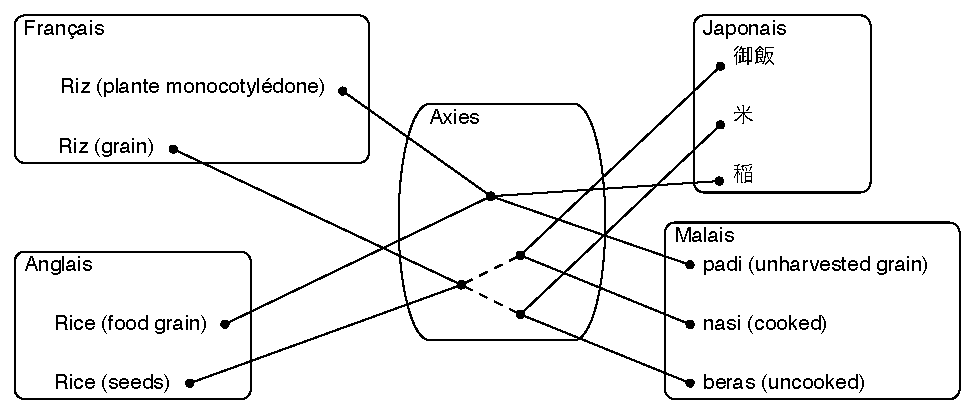
\includegraphics[width=\linewidth]{figs/axies.pdf}
}

\frame{
  \frametitle{Architecture of the Data}
  \framesubtitle{A microstructure inspired by Mel'\v{c}uk's ECD and Polguère's DICO}
  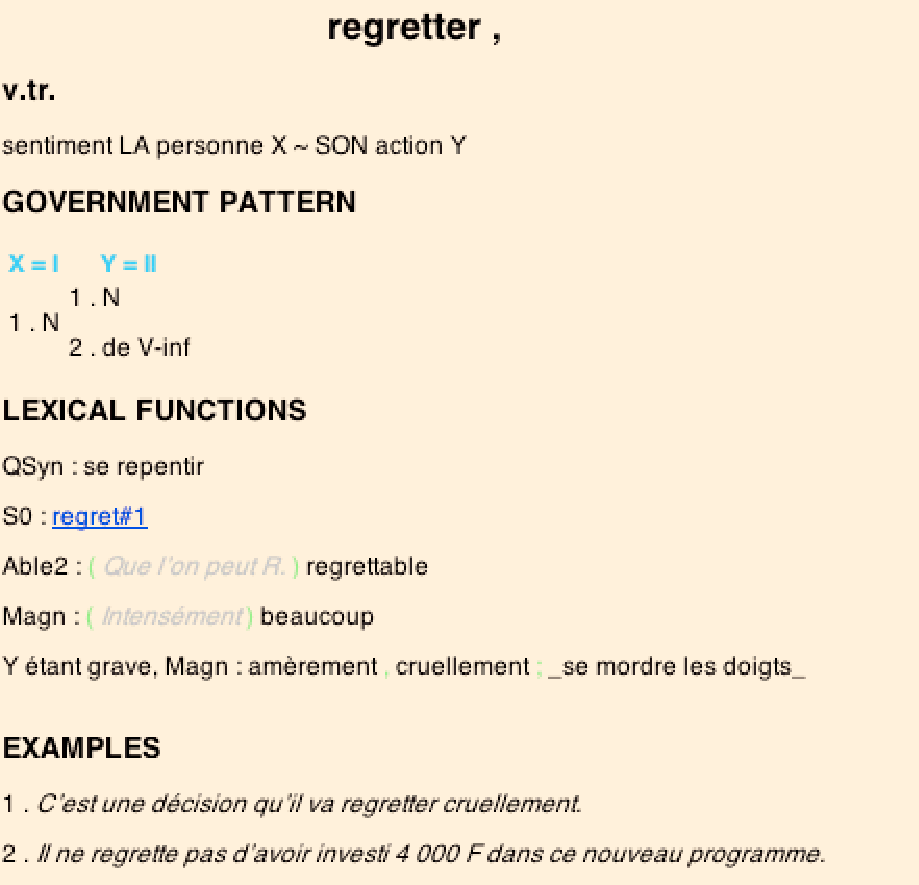
\includegraphics[height=7cm]{figs/regretter-expanded.pdf}
}

\frame{
\frametitle{Mel'\v{c}uk's ECD and Lexical Functions: Motivations}
\begin{tabular}{lll}
  gros fumeur & lit. trans. & big smoker\\
& actual trans. & heavy smoker
\end{tabular}

An MT system has to identify that \alert{gros fumeur} 
is a collocation, something between a free 
combination and a full idiom
}

\frame{\frametitle{Mel'\v{c}uk's ECD and Lexical Functions}

Following Meaning-Text terminology, we call 
\alert{collocation} a linguistic expression made up of 
two components: 

\begin{itemize}
\item the base of the collocation: a full lexical unit which 
is ``freely'' chosen by the speaker on the basis of 
its meaning (e.g. ‘smoker’ $\rightarrow$ smoker); 
\item the collocate: a lexical unit or a multilexical 
expression which is chosen in a (partially) arbitrary 
way to express a given meaning and/or a 
grammatical structure contingent upon the choice 
of the base (e.g. ‘intense’ $\rightarrow$ heavy).

\end{itemize}
}

\frame{\frametitle{Mel'\v{c}uk's ECD and Lexical Functions}
Rich bilingual dictionary 
\begin{itemize}
\item fumeur $\Leftrightarrow$ smoker 
\item gros fumeur $\Leftrightarrow$ heavy smoker 
\end{itemize}

~

Minimal bilingual dictionary 
\begin{itemize}
\item fumeur $\Leftrightarrow$ smoker  
\end{itemize}

 + rich monolingual dictionaries 
 \begin{itemize}
 \item intensification(fumeur) = gros  
 \item intensification(smoker) = heavy
 \end{itemize}
}

\frame{\frametitle{Mel'\v{c}uk's ECD and Lexical Functions}

Collocations are numerous and various in 
nature. 

~

E.g.: COLÈRE ‘anger’
\begin{itemize}
\item colère aveugle/noire, lit. ‘blind/black anger’ 
\item colère sourde/froide, lit. ‘deaf/cold anger’ 
\item fou/ivre de colère, lit. ‘mad/drunk of anger’ 
\item rouge/blanc de colère, lit. ‘red/white of anger’ 
\end{itemize}
etc.
}

\frame{\frametitle{Mel'\v{c}uk's ECD and Lexical Functions: Collocation and Semantic Derivation}

Intensification of rain: 
\begin{itemize}
\item torrential (collocate)
\item downpour (semantic derivation) 
\item torrential rain ~ downpour 
\end{itemize}

Semantic derivations 
\begin{itemize}
\item (quasi)synonymy/antonymy 
\item verbal, nominal, adjectival or adverbial derivations 
\item name of a participant or circonstant, e.g. crime is linked to 
author [of a crime] or criminal, victim, instrument [of a crime], etc. 
\end{itemize}
 
Both types of lexical relation could and should 
be encoded by the same conceptual device
}

\frame{\frametitle{Mel'\v{c}uk's ECD and Lexical Functions: Collocations as Functions}

Concept of LF: Zholkovskij \& Mel'\v{c}uk 1965 
 
Base-collocate relations are \alert{oriented} 

~

\centering{
  \begin{tabular}{ccc}
Magn & (rain) & = torrential\\
function&(base)& = collocate   
 \end{tabular}
}
}

\frame{
  \frametitle{Architecture of the Data}
  \framesubtitle{A microstructure inspired by Mel'\v{c}uk's ECD and Polguère's DICO}
  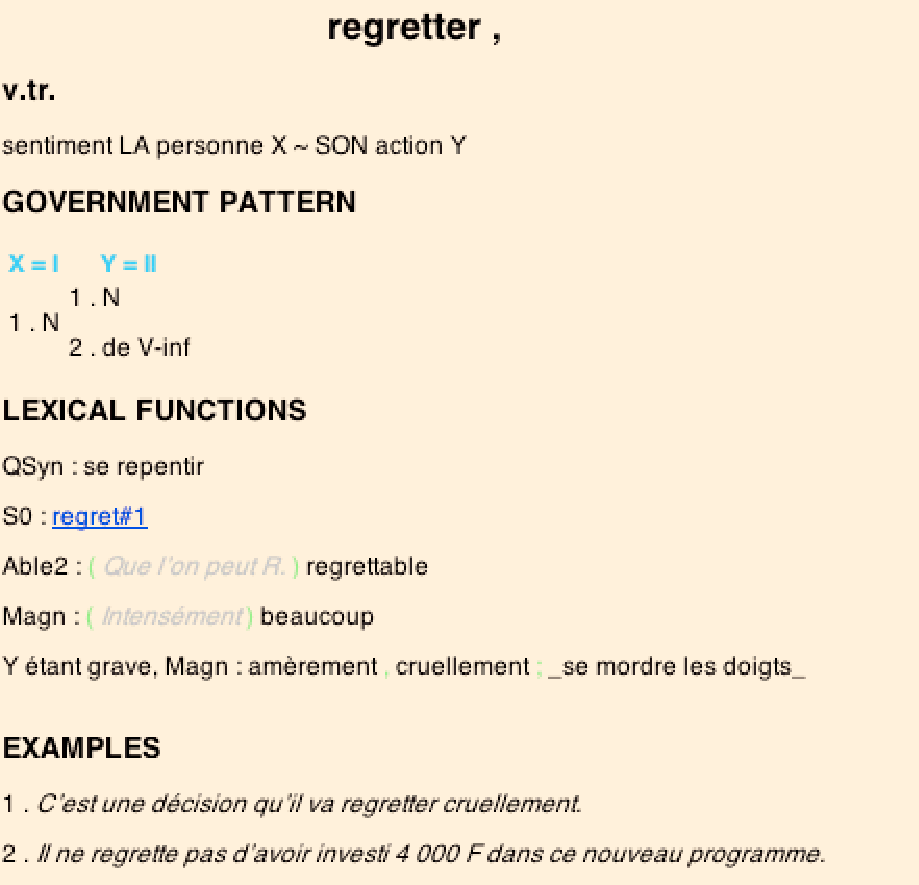
\includegraphics[height=7cm]{figs/regretter-expanded.pdf}
}

\section{The LexALP project}
\frame{
  \frametitle{LexALP Project Motivations}
  \begin{itemize}
    \item The Alpine Convention gathers European countries who agrees on certain rules on
    \begin{itemize}
       \item environment, spatial planning, transport infrastructure, \ldots
       \item for the Alpine Space (from Monaco to Slovenia)
    \end{itemize}
   %\includegraphics<1>[width=\linewidth]{alps.jpg}

    \pause
    \item But these rules need to be carefully worded
     \begin{itemize}
       \item and negotiators often disagree on the wording of documents
       \item (half the time of meetings spent in discussions about the minutes)
    \end{itemize}
    \pause
    \item Moreover, these rules should be implemented by participating states
    \begin{itemize}
       \item hence, adequate terminology should be used in each country
       \item to correctly refer to existing laws
    \end{itemize}
  \end{itemize}
}

\frame{
  \frametitle{Examples of \alert{Legal} Language Problems}
    \begin{itemize}
   \item Different terms for the same meaning
  \begin{itemize}
  \item \alert{chien drogue} is used in European texts\ldots
  \item \ldots when texts from France use \alert{chien renifleur}
  \end{itemize}
  \pause
   \item Different meanings for the same term
  \begin{itemize}
  \item \alert{Landeshauptmann} in Bolzano (Italy)\ldots
  \item \ldots has much less power than an Austrian \alert{Landeshauptmann}
  \end{itemize}
  \pause
   \item Superficial translation leads to legal differences
  \begin{itemize}
  \item \alert{elezione suppletiva} is commonly 
held whenever an elected deputy or senator either resigns or 
dies
\item \alert{Ersatzwahlen} are very rare, as in Germany the first non-elected candidate is called to parliament 
  \end{itemize}

  \end{itemize}
  }

\frame{
  \frametitle{A Legal Language Harmonisation System}
  \framesubtitle{For Environment and Spatial Planning within the Multilingual Alps}

  \begin{itemize}
  \item Describe legal terminology of the Alpine Convention (in its four languages)
  \item Harmonise it
  \end{itemize}
  \pause
  \alert{$\rightarrow$ For use by negotiators and translators of the Alpine Convention}
  \pause
  \begin{itemize}
  \item Link it to the equivalent/near-equivalent terms in the national legal systems
  \end{itemize}
  \pause
  \alert{$\rightarrow$ For use by jurist who will implement the law in other legal systems}
}

\frame{
\frametitle<1,3->{LexALP Bibliographic Database}
     \includegraphics<2>[width=\linewidth]{figs/subfield_structure_en.jpg}
     \includegraphics<4>[width=.7\linewidth]{figs/bib_details_crop.jpg}

\only<1,3>{\begin{itemize}
\item Legal documents are collected (in raw text format)
\item Along with their classification:
\begin{itemize}
\item title of the document
\item short title of the document
\item abbreviation of the document
\item language
\item legal system
\item legal hierarchy (e.g. national, regional, supranational)
\item legal text type
\item translation status (original or translation)
\item subfield
\item<3,5> + additional fields depending on the legal system
\end{itemize} 
\end{itemize}
}
\only<5>{$\rightarrow$ this leads to a bibliographic database\\
that contains documents of the corpus, \\
but also documents that are not available in the corpus\\
~\\
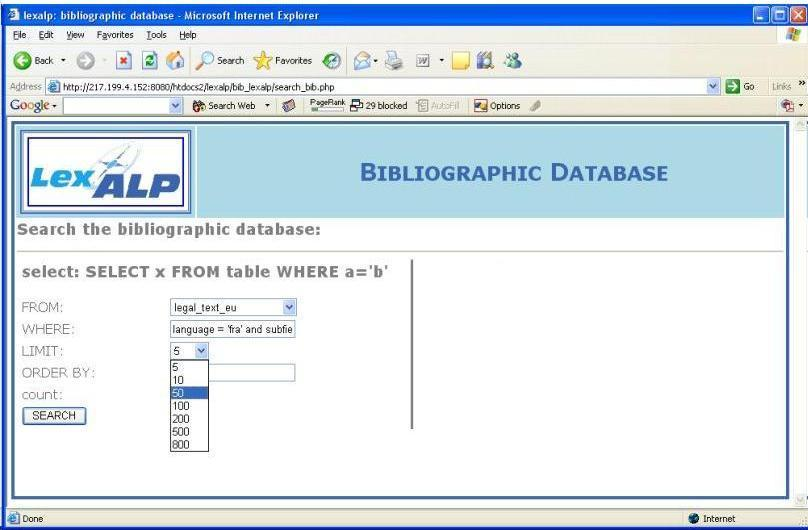
\includegraphics[width=.6\linewidth]{figs/search_bib.jpg}}
}


\frame{
\frametitle{LexALP Document Structure}
\begin{itemize}
\item The documents of each legal system are automatically annotated by the means of several scripts. 
\item The annotation is done on a structural level taking into account textual subdivisions (sentences etc.) as well as subdivisions particular to legal documents (chapters, articles, ...).
\end{itemize}
\begin{alltt}\scriptsize
<div type="section" id="FR\_U3\_ENVIR-PL-L4-T2-44-14-11.xml.b.c0.se3">\\
~<p id="FR\_U3\_ENVIR-PL-L4-T2-44-14-11.xml.b.c0.se3.p0">\\
~~<title id="FR\_U3\_ENVIR-PL-L4-T2-44-14-11.xml.b.c0.se3.p0.ti1">\\
~~~Article L420-3\\
~~~(Loi nº 2005-157 du 23 février 2005 art. 150, art. 151, \\
~~~~art. 154 Journal Officiel du 24 février 2005)\\
~~</title></p>\\
~<p id="FR\_U3\_ENVIR-PL-L4-T2-44-14-11.xml.b.c0.se3.p1">\\
~~<s id="FR\_U3\_ENVIR-PL-L4-T2-44-14-11.xml.b.c0.se3.p1.s1">\\
~~~Constitue un acte de chasse tout acte volontaire lié à la recherche, \\
~~~à la poursuite ou à l'attente du gibier ayant pour but ou pour résultat \\
~~~la capture ou la mort de celui-ci.\\
~~</s></p>\\
\end{alltt}
}

\frame{
\frametitle{LexALP Corpus Structure}
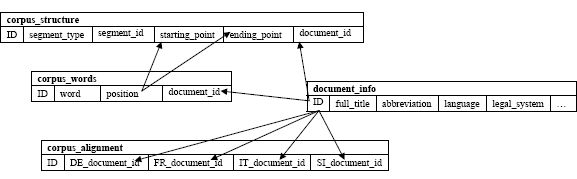
\includegraphics[width=\linewidth]{figs/database_table_linking.jpg}
}

\frame{
\frametitle{LexALP Corpus Search}
\includegraphics<1>[width=\linewidth]{figs/corpus_fuzzy_search_crop.jpg}
\includegraphics<2>[width=\linewidth]{figs/output_fuzzy_search.jpg}
}

\pgfdeclareimage[height=.75em]{fr}{figs/FR}
\pgfdeclareimage[height=.75em]{ac}{figs/AC}
\pgfdeclareimage[height=.75em]{eu}{figs/EU}

\frame{
\frametitle{The LexALP term bank}
\begin{itemize}
\item The term bank is a collection of ``\alert{lexies}''
\item Each lexie represents a \alert{word sense} (or acceptation) of the domain
  \begin{itemize}
  \item ex: \pgfuseimage{fr}~principe de précaution $\neq$ \pgfuseimage{ac}~principe de précaution
  \item ex: \pgfuseimage{fr}~chien renifleur $\neq$ \pgfuseimage{eu}~chien drogue
  \end{itemize}
\item Lexies are linked by interlingual relations called ``\alert{axies}''
\end{itemize}
}

\frame{
  \frametitle{Building the LexALP Term Bank}
  \framesubtitle{Monolingual step}
     \includegraphics<2>[width=\linewidth]{figs/trafic_intra-alpin-lexies.pdf}

  \only<1>{
   \begin{enumerate}
    \item<1> Develop a quadrilingual term bank
    \begin{itemize}
       \item French, German, Italian and Slovenian
       \item based on Alpine Convention texts
    \end{itemize}
    \end{enumerate}
  }
}

\frame{
  \frametitle{LexALP Microstructure}
     \includegraphics<1>[width=\linewidth]{figs/edition1.jpg}
     \includegraphics<2>[width=\linewidth]{figs/edition2.jpg}
}


\frame{
  \frametitle{Building the LexALP Term Bank}
  \framesubtitle{Multilingual steps}
     \includegraphics<2>[width=\linewidth]{figs/trafic_intra-alpin-lexies.pdf}
     \includegraphics<4>[width=\linewidth]{figs/trafic_intra-alpin.pdf}
     \includegraphics<6>[width=\linewidth]{figs/trafic_intra-alpin_harmonized.pdf}
     \includegraphics<8>[width=\linewidth]{figs/principe_precaution.pdf}

  \only<1,3,5,7>{
   \begin{itemize}
    \item<1,3,5,7> Develop a quadrilingual term bank
    \begin{itemize}
       \item French, German, Italian and Slovenian
       \item based on Alpine Convention texts
    \end{itemize}
    \item<3,5,7> Link equivalents on the Alpine Convention level
   \item<5,7> Harmonize the terms at the Alpine Convention level
    \item<7> Link these terms with related terms defined in national legal texts
    \begin{itemize}
       \item Austria, France, Germany, Italy, Slovenia, Switzerland (Monaco, Liechtenstein)
       \item based on national/regional legal texts
    \end{itemize}
  \end{itemize}
  }
  
  \only<3>{\alert{$\rightarrow$ We use "axies" (with an e) for the multilingual interoperability}} 
}


%----------------------------------
\section{Summary}
\frame{\frametitle{What have we learned until then?}
  \begin{itemize}
  \item many different lexical resources do exist nowadays,
  \item many more will be built in the future,
    \pause
  \item each lexical database defines its own \alert{macro-structure}
    \begin{itemize}
    \item monolingual: usually 1 volume for 1 language,
    \item bilingual: usually 2 independent volumes ($l_1 \rightarrow l_2$ + $l_2 \rightarrow l_1$)  
    \item multi-bilingual: either same as bilingual, but with more independent volumes, or a set of monolingual volume plus a set of bilingual links volumes
    \item fork dictionaries: either a unique volume or monolingual volume + translation links volumes, only one source language,
    \item multilingual: using monolingual volumes + one central, pivot volume;
    \end{itemize}
    \pause
  \item each lexical database defines its own \alert{micro-structure}
    \begin{itemize}
    \item Here, there is no real limit to the imagination of lexicologists...
    \end{itemize}
  \end{itemize}
}

% Micro structure, macrostructure
% classes of MLDB (monolingual, bilingual, multi-bilingual, fork dictionaries, pivot dictionaries (kind of pivots used).

\part{Building MLDB: a mixture of Linguistic and Computer Problems}
\frame{\partpage}

\section{Analysing the problem}

\frame{
  \frametitle{Analysing the problem: economic aspects}
  \begin{itemize}
    \item Building a rich bilingual dictionary is expensive...
    \pause
    \begin{itemize}
      \item ex: EDR: $>350000$ words in Japanese-English
      \item $\rightarrow 14305$ M\yen
      \item $\rightarrow$ {\bfseries VERY} expensive
    \end{itemize}
    \pause
    \item How can we reduce the costs ?
    \begin{itemize}
       \item Share the costs $\rightarrow$ using a a general structure, adaptable to many applications
       \item Reduce the costs $\rightarrow$ reusing existing data whenever possible, implementing adequate tools
       \item Federate the costs $\rightarrow$ allow anyone to contribute and use the data
    \end{itemize}
  \end{itemize}
}

\frame{
\frametitle{Analysing the Problem: competences}

\begin{itemize}
\item Dictionaries play a central role in human and artificial Language Processing tasks
\item But building a dictionary is highly difficult
\pause
\item It requires linguistic skills
\begin{itemize}
\item to define a valid structure
\item and produce correct entries
\end{itemize}
\pause
\item It requires rigourous organisational skills
\begin{itemize}
\item to manage different lexicographers
\item with different skills
\end{itemize}
\pause
\item It requires computational skill
\begin{itemize}
\item to ensure well-formedness/validity of the entries
\item to avoid losing data by mistake
\end{itemize}
\end{itemize}
\only<5>{$\rightarrow$ The linguistic skill will always be necessary}
\only<6>{$\rightarrow$ \alert{But the other skills should be optional}}
}

\frame{
\frametitle{Analysing the Problem: requirements}
\begin{itemize}
\item For this, we need a dictionary building system
\item which allows team work
\item which provides integrity of data (backup/history/rollback...)
\item which is customisable 
\begin{itemize}
\item to accept different micro-structures (structure of each entry)
\item to accept different macro-structure (monolingual, bilingual, multi-bilingual, pivot based, \ldots)
\end{itemize}
\item with minimal knowledge of computer science
\end{itemize}
\only<2>{$\rightarrow$ No system was able to fulfil all these requirements}
\only<3>{$\rightarrow$ \alert{We developed the Jibiki plateform}}
}

% How to structure them ?
% How to build them ?
% How to use them ?
% How to make them interoperate ?

\section{Jibiki: an open source plateform for MLDB collaborative building}



\frame{
  \frametitle{The Jibiki platform}
  \framesubtitle{A community web site development platform offering several services}
  \begin{itemize}
    \item Dictionary access for many different dictionaries
    \item Dictionary edition for selected dictionaries
    \item Community services
    \begin{itemize}
       \item Mailing list archive
       \item Documentation pool shared by partners
    \end{itemize}
  \end{itemize}
}


\frame{
  \frametitle{Implementation}
   \includegraphics<1>[width=\linewidth]{figs/Architecture-serveur_en.pdf}
}

\section{Services provided and how they work}


\frame{
  \frametitle{The LexALP website}
  \begin{itemize}
    \item We used the Jibiki plateform to set-up LexALP website
    \item it offers access to the term bank...
    \item and allows for dictionary edition
  \end{itemize}
}

\frame{
  \frametitle{The LexALP website}
    \framesubtitle{Simple dictionary access}
     \includegraphics<1>[width=.3\linewidth]{figs/simple_search.png}
     \includegraphics<2>[width=\linewidth]{figs/result.png}
}


\frame{
  \frametitle{The LexALP website}
    \framesubtitle{Edit terms and interlingual links  \hyperlink{sizenote}{\beamergotobutton{Side note}}}

     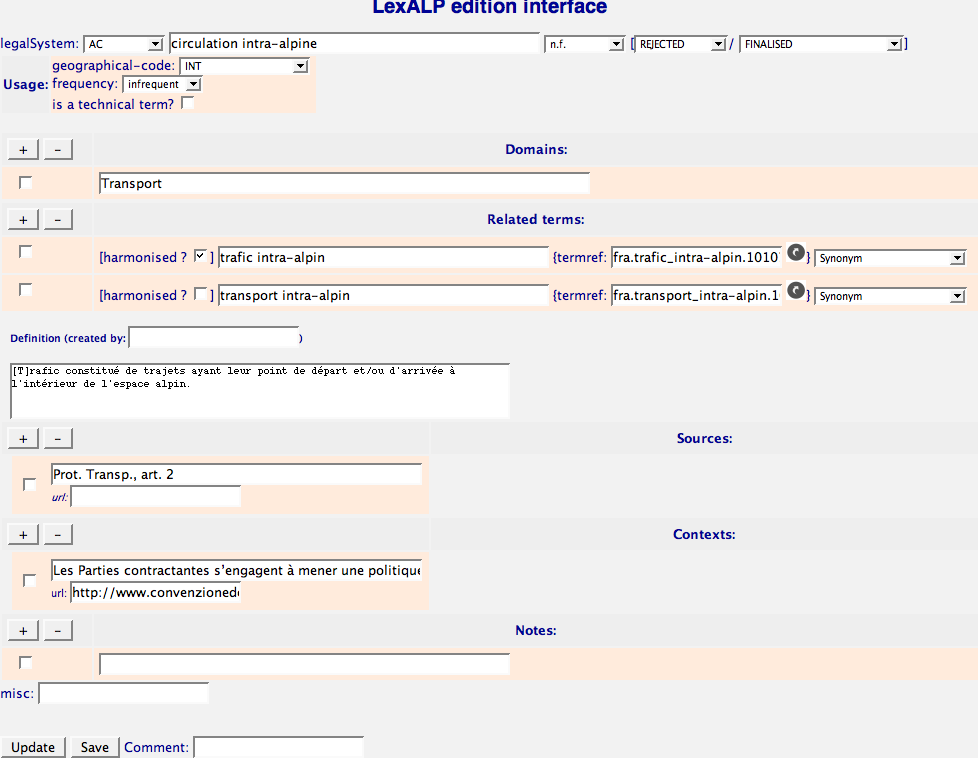
\includegraphics[width=\linewidth]{figs/edition_interface.png}
     \hypertarget{illustration}{}
}


\frame{
  \frametitle{What is the necessary work for this ?}
  \framesubtitle{Providing dictionary access}
     \includegraphics<3>[width=\linewidth]{figs/principe_precaution_xml.pdf}
     \includegraphics<5>[width=\linewidth]{figs/principe_precaution_xml_cdm.pdf}

  \only<1,2,4,6>{
   \begin{enumerate}
    \item<1,2,4,6> Decide on the structure of your lexical database
    \begin{itemize}
       \item Monolingual, bilingual, multi-bilingual, interlingual
       \item $\Rightarrow$ Here, we chose an interlingual approach
       \item $\Rightarrow$ with 5 monolingual dictionaries and 1 pivot
    \end{itemize}
   \item<2,4,6> Then, decide on the structure of your dictionary 
   \begin{itemize}
       \item Your only constraint is: use an XML structure
    \end{itemize}
    \item<4,6> Identify your pieces of informations
    \begin{itemize}
       \item by associating elements in your structures with elements of a simple structure\ldots
       \item \ldots called the Common Dictionary Markup structure
       \item association is done with simple XPaths
    \end{itemize}
    \item<6> Provide a presentation form for your users
    \begin{itemize}
       \item by way of a simple XML stylesheet (producing xhtml from the xml structure)
    \end{itemize}

  \end{enumerate}}
}

\frame{
  \frametitle{What is the necessary work for this ?}
    \framesubtitle{Providing dictionary Editing}

  \begin{enumerate}
    \item Define the XML schema of your structure
    \pause
    \item Provide an empty structure bearing default values
    \pause
    \item Let the system generate a default interface
    \pause
    \item Customise it to fit your user needs
    \begin{itemize}
    \item you can hide the information you don't want your contributors to see
    \end{itemize}
  \end{enumerate}

}

\part{Other approaches to dictionary structuration}

\frame{
\partpage
}

\frame{  
\frametitle{Structuring the dictionary as a graph}
 \begin{enumerate}
    \item No more "entry" (but you need to type your nodes somehow)
    \pause
    \item May be represented in RDF
    \pause
    \item Leads to the Lexical Web
    \pause
    \item Properties of arcs may be used to rationalize the MLDB data
    \begin{itemize}
    \item you can still provide a "natural" way to \emph{present} your data
    \end{itemize}
  \end{enumerate}
}

\frame{  
\frametitle{Example: Mel'\v{c}uk ECD as a Lexical System (A. Polguère)}

     \includegraphics<1>[width=\linewidth]{img/Ploguere_LS_rancune.png}
     \includegraphics<2>[width=\linewidth]{img/Polguere_LS_chat.png}

}

\frame{  
\frametitle{Example: Wiktinary data as a graph (G. Sérasset)}

     \includegraphics<1>[width=\linewidth]{img/wkt-chat1.png}
     \includegraphics<2>[width=\linewidth]{img/wkt-chat.pdf}

}

\frame{  
\frametitle{Advantage: Crowdsourcing or Games With A Purpose}

    \begin{enumerate}
    \item As data is "split" in atomic units (relations)...
    \item ... contributing to data is easier...
    \item ... and does not require to grasp the structure of a whole entry.
    \pause
    \item Hence, it is possible to add small parts without any lexicography knowledge
    \begin{itemize}
    \item $\rightarrow$ http://jeuxdemots.org
    \end{itemize}
  \end{enumerate}

}

\end{document}


\part{A Step by Step tutorial on jibiki}
\frame{\partpage}


\part{An Autopsy of Existing Dictionaries Build with Jibiki}
\frame{\partpage}


\part{Future works}

\section{Making Structures Inter-operate}
\frame{}

\subsection{LMF common Model}

\subsection{improving CDM}





